\documentclass[11pt,twoside=false,open=any]{scrbook}

\usepackage[utf8]{inputenc}
\usepackage[ngerman]{babel}
\usepackage{skript2016}

\usepackage{siunitx}
\usepackage{wrapfig}
\usepackage{nicefrac}


\begin{document}
\title{Skript zur Elektrostatik 1}

\author{Matthias Heimberg}
\publishers{Gymnasium Oberaargau}
\date{Sekunda, 2016}

\begingroup
 \makeatletter
 \@titlepagetrue
 \maketitle
\endgroup
\newpage

\newcounter{aufgaben}
\tableofcontents
\newpage
\chapter{Statische Elektrizität und Ladung} 
Wir wissen heute, dass sämtliche Objekte um uns aus Atomen bestehen. Diese Atome bestehen ihrerseits aus einem Kern und der ihn umgebenden Elektronenwolke. Im Kern finden wir elektrisch geladenen Protonen und elektrisch neutrale Neutronen. Die Elektronenwolke besteht aus elektrisch geladenen Elektronen. Wir bezeichnen die Ladung der Protonen als die \textbf{positive Ladung} und die der Elektronen als die \textbf{negative Ladung}. 

\begin{center}
   \setlength{\fboxrule}{2pt}
   \fcolorbox{black}{gray!10}{
\begin{minipage}{\textwidth}
\paragraph{Definition}

Ladung ist eine physikalische Eigenschaft von Objekten, die dazu führt, dass diese von anderen geladenen Objekten angezogen oder abgestossen werden. Jedes geladene Objekt erzeugt und wird beeinflusst von einer Kraft die wir die elektromagnetische Kraft nennen.

\end{minipage}
}
\end{center}

\section{Proton und Elektron}
Nahezu jede Ladung in der Natur besteht aus Elektronen und/oder Protonen (es existieren noch andere Teilchen, die Ladung tragen, diese sind aber selten und sind nicht lange stabil).

Die Ladungen von Elektron und Proton sind gleich im Betrag, aber mit entgegengesetztem Vorzeichen. Alle Ladungen in der Natur sind \textbf{ganzzahlige Vielfache} dieser elementaren Ladungen. Wir bezeichnen diese \textbf{Elementarladung mit:}

\[ | q_{e} | = \SI{1.60E-19}{\coulomb} \]

Das Symbol $q$ oder $Q$ wird üblicherweise für die Grösse der Ladung verwendet.
Elektronen scheinen keine innere Struktur zu besitzen, wir nehmen heute an, dass sie punktförmig sind. Im Gegensatz dazu lassen Streuexperimente an Protonen darauf schliessen, dass diese in ihrem Innern aus punktförmigen Teilchen aufgebaut sind; diese Sub-Teilchen, Quarks genannt, wurden noch nie direkt beobachtet. Man nimmt heute an, dass die Quarks Ladungen von entweder $-\frac{1}{3}$ oder $\frac{2}{3}$ tragen (gemessen in Elementarladungen). Die Quarks bilden vermutlich die ultimative Substruktur der Materie, d.h. sie sind ihrerseits elementar (ohne innere Struktur). Für ein Proton gilt also:
\[ q_{Proton} = \frac{2}{3}q_{e} + \frac{2}{3}q_{e} -\frac{1}{3}q_{e} \]
\section{Die Ladungserhaltung}
Wenn ein Objekt geladen wird, wird nicht wirklich eine Ladung erzeugt. Die in den Atomen bereits vorhandenen Ladungen werden bei diesem Vorgang voneinander getrennt und herumbewegt. Tatsächlich bleibt die \textbf{Gesamtladung} bei sämtlichen Vorgängen erhalten:
\begin{center}
   \setlength{\fboxrule}{3pt}
   \fcolorbox{black}{gray!10}{
\begin{minipage}{\textwidth}
Ladungserhaltung:
\vspace{2cm}

\end{minipage}
}
\end{center}

In etwas exotischeren Beispielen, zum Beispiel in Teilchenbeschleunigern, kann Masse $\Delta m$ aus Energie entstehen (nach $\Delta m = \frac{E}{c^2}$). Es kann vorkommen, dass diese Masse geladen ist, zum Beispiel wenn ein Elektron entsteht. Wenn nun aber ein geladenen Teilchen entsteht, dann muss gleichzeitig ein entgegengesetzt geladenes Teilchen entstehen, damit die Gesamtladung konstant (Null) bleibt. Üblicherweise bilden die beiden Teilchen ein Materie-Antimaterie-Paar. Zum Beispiel würde gleichzeitig mit dem Elektron auch ein Anti-Elektron entstehen. Das Anti-Elektron besitzt eine positive Ladung (es wird Positron genannt), und somit ist die \textbf{Gesamtladung} der erzeugten Masse Null. Zu jedem Teilchen existiert ein Antiteilchen mit der entgegengesetzten Ladung. Wenn Materie und Antimaterie Teilchen zusammengebracht werden, so annihilieren sie sich gegenseitig. Annihilieren bedeutet hier, dass die gesamte Masse der beiden Teilchen in Energie verwandelt wird (auch beschreiben durch $\Delta m = \frac{E}{c^2}$). Da die beiden Teilchen eine entgegengesetzte Ladung besitzen, ist die Gesamtladung vor und nach der Annihilation Null, die Gesamtladung ist auch hier erhalten. 

\begin{center}
   \setlength{\fboxrule}{2pt}
   \fcolorbox{gray!30}{gray!10}{
\begin{minipage}{\textwidth}
\paragraph{Aufgaben}
\begin{enumerate}
\item Die meisten Objekte bestehen aus einer extrem hohen Anzahl von geladenen Teilchen, weshalb beobachten wir dann nicht bei allen Objekten statische Elektrizität?
\item Weshalb enthalten die meisten Objekte gleich viele negative wie positive Ladungen?
\item Gewöhnliche statische Elektrizität funktioniert mit Ladungen im Bereich von Nano- bis Mikrocoulomb. Wie viele Elektronen werden benötigt um eine Ladung von $-\SI{2.00}{\nano \coulomb}$ zu erstellen? Wie viele Elektronen müssen entfernt werden um eine Ladung von \SI{0.500}{\micro \coulomb} zu erhalten?
\item Wenn in einem Tag \SI{1.80E20}{} Elektronen durch einen Taschenrechner bewegt werden, wie viele Coulomb Ladung wurden dann bewegt?
\item Um ein Auto zu starten, bewegt die Autobatterie \SI{3.75E21}{} Elektronen durch die Zündkerze. Wie viele Coulomb Ladung wurden bewegt?
\item In einem Blitz wird eine Ladung \SI{40.0}{\coulomb} bewegt. Wie viele Elementarladungen $|q_{e}|$ sind dies?
\setcounter{aufgaben}{\value{enumi}}
\end{enumerate}
\end{minipage}
}
\end{center}


\chapter{Leiter und Isolatoren}

Einige Substanzen wie zum Beispiel Metalle und Salzwasser erlauben es den Ladungen, sich relativ frei hindurchzubewegen. Einige der Elektronen in Metallen und ähnlichen Leitern sind nicht an individuelle Atome im Material gebunden. Diese \textbf{freien Elektronen} können sich ähnlich durch das Material bewegen, wie Luft durch losen Sand. All diese Substanzen, die freie Elektronen besitzen und in denen sich Ladungen relativ frei bewegen können, nennen wir \textbf{Leiter}. Die sich bewegenden Elektronen werden zwar mit den fixen Atomen und Molekülen des Materials kollidieren und verlieren dabei etwas Energie, aber sie können sich in dem Leiter bewegen. Leiter in denen sich die Ladungen ohne Energieverlust bewegen können, nennen wir Supraleiter.
Salzwasser und andere ähnliche leitende Materialien enthalten freie Ionen die sich durch das Material bewegen können. Ein Ion ist ein Atom oder Molekül mit einer positiven oder negativen Gesamtladung (Ladungsungleichgewicht). Mit anderen Worten: Die Anzahl der Elektronen stimmt nicht mit der Anzahl der Protonen überein.


Durch andere Substanzen wie zum Beispiel Glas oder Keramik können sich keine Ladungen bewegen. Diese Substanzen nennen wir \textbf{Isolatoren} oder Nichtleiter. Elektronen und Ionen in Isolatoren sind in der Struktur des Materials gebunden und können sich nicht einfach so bewegen (ungefähr \SI{10E23}{} mal langsamer als in Leitern). Reines Wasser und trockenes Tafelsalz sind Isolatoren, gelöstes Salz und Salzwasser hingegen sind Leiter. 

\section{Laden eines Objektes durch Kontakt}
\begin{figure}[h]
\centering
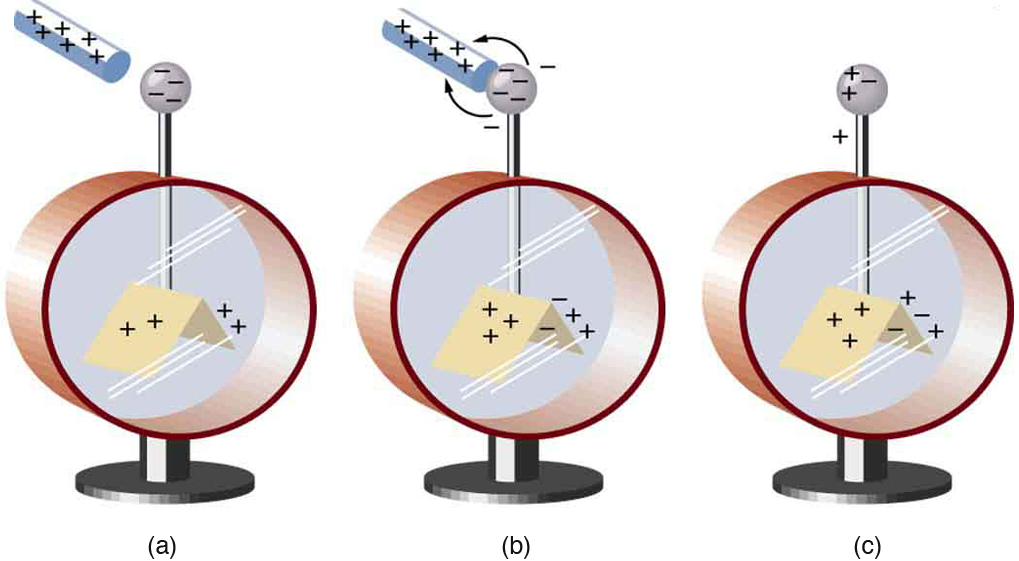
\includegraphics[width=10cm]{elektroskop1.jpg}
\caption{(a) Ein positiv geladener Glasstab wird in die Nähe des ungeladenen Elektroskops gebracht. Elektronen des Elektroskopes werden in den oberen Teil gezogen und hinterlassen unten eine positive Ladung. (b) Wenn der Stab das Elektroskpo berührt, werden Elektronen auf den Stab übergehen und verringern somit die Gesamtladung des Glasstabes aber hinterlassen das Elektroskop mit einer positiven Gesamtladung. (c) Die überschüssige Ladungen verteilt sich gleichmässig im Elektroskop}
\label{fig:elektroskop1}
\end{figure}

Die Abbildung \ref{fig:elektroskop1} zeigt ein Elektroskop, das durch die Berührung mit einem positiv geladenen Glasstab geladen wird. Da der Glasstab ein Isolator ist, muss er das Elektroskop tatsächlich berühren, um ihm Ladungen zu entziehen oder Ladungen aufzubringen. Da die Elektronenen sich nur im Metall bewegen können, werden die Elektronen im Elektroskop nach oben bewegt. Dort werden einige davon bei der Berührung auf den Glasstab übergehen und hinterlassen damir das Elektroskop mit einer positiven Gesamtladung. \textbf{Elektrostatische Abstossung} führt dazu, dass sich die Nadel im Elektroskop bewegt. 

\section{Laden eines Objektes durch Influenz} %http://cnx.org/contents/Ax2o07Ul@9.4:8vWesjNz@4/Conductors-and-Insulators
Um ein Objekt elektrisch aufzuladen, benötigt man keine direkte Berührung mit einer Ladung. Die Abbildung \ref{fig:influenz1} zeigt eine Methode durch \textbf{Influenz}. Zwei neutrale Metallkugeln berühren sich, sind aber vom Rest der Welt isoliert. 
\begin{figure}[h]
\centering
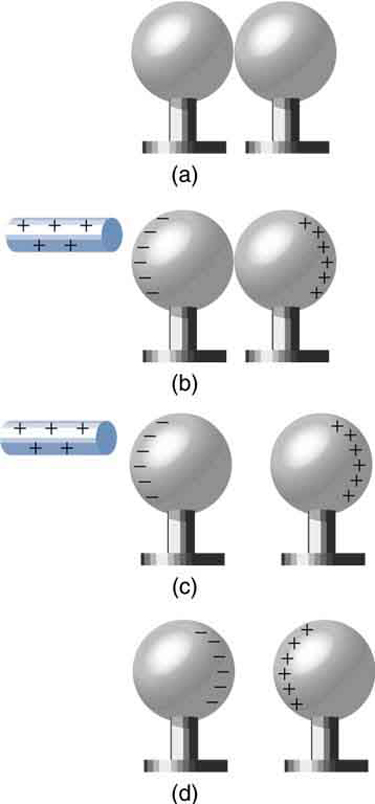
\includegraphics[width=4.5cm]{influenz1.jpg}
\caption{Laden durch Influenz: (a) Zwei ungeladenen Metallkugeln berühren sich, sind aber vom Rest der Welt isoliert. (b) Ein positiv geladener Glasstab wird in die Nähe der linken Kugel gebracht. Die negativen Ladungen in der Kugel werden angezogen} 
\label{fig:influenz1}
\end{figure}









\chapter{Das Coulomb-Gesetz und das elektrische Feld}
Die Coulombkräfte zwischen elektrischen Ladungen wirken, ohne dass sich die Ladungen be-rühren. Wir nennen dieses Phänomen \textbf{Fernwirkung} von Kräften. Wir haben bereits eine fernwirkende Kraft kennen gelernt: Die Gravitationskraft. Die Gleichung der Gravitationskraft (\ref{FG}) zwischen zwei Massen besitzt den gleichen Aufbau wie die Coulomb-Gleichung (\ref{FC}) für die elektrische Kraft zwischen zwei (punktförmigen) Ladungen:

    \begin{equation}
	\label{FG}
		F_{G} = G \cdot \frac{m_{1} \cdot m_{2}}{r^{2}};
	\end{equation}
 
	\begin{equation}
	\label{FC}
		F_{C} = k \cdot \frac{Q_{1} \cdot Q_{2}}{r^{2}} 
	\end{equation}

Die beiden Kräfte zeigen ein fast identisches Verhalten, unterschiedlich ist ihre Stärke und die Tatsache, dass die Gravitationskraft eine ausschliesslich \textcolor{black}{anziehende} Kraft ist. Für keine der beiden Kräfte ist ein Medium notwendig, das heisst, wir können diese auch nachweisen, wenn zwischen den Körpern ein Vakuum herrscht. 

Bisher haben wir diese Kraftwirkungen mittels der sogenannten \textbf{Fernwirkungstheorie} beschrieben: Betrachten wir dazu ein einfaches Beispiel aus dem Physikunterricht (siehe Abbildung \ref{Bsp1}): Eine positiv aufgeladene Kugel hängt an einem Isolierfaden.
Bringt man in ihre Nähe die ungeladene Haube des Bandgenerators, so wird die Kugel zunächst geringfügig von der neutralen Haube angezogen. Lädt man nun die Haube des Bandgenerators positiv auf, so wird die Kugel nach rechts bewegt, da sich gleichnamig geladene Körper abstossen. Als Ursache für die Auslenkung der Kugel wird die in einer gewissen Entfernung  angeordnete positiv geladene Haube des Bandgenerators angesehen. 

\begin{figure}[h]
\begin{center}
\begin{tikzpicture}[scale=0.6]
\draw[ball color=white, shading=ball] (0,0) node{$+$ $+$ $+$} circle (1.5cm) node[below=1cm] {Bandgenerator};
\draw (4.5,0) -- (3.5,6);
\draw[dashed] (3.5,6) -- (3.5,0);
\draw[ball color=white, shading=ball] (4.5,0) node {$+$} circle (5mm);
\draw[->,draw=red,thick] (4.5,0) -- node[below,style=red] {$\vec{F}_{C}$} (6.5,0);
\end{tikzpicture}
\caption{Eine positiv geladene Kugel wird von der gleichnamig geladenen Haube des Bandgenerators abgestossen}
\label{Bsp1}
\end{center}
\end{figure}

\section{Das elektrische Feld (Nahwirkungstheorie)}
In der Physik benützen wir den Begriff \textbf{``Feld''} um diese Kraftwirkungen ohne Fernwirkung zu beschreiben. Der amerikanische Physiker Richard Feynman\footnote{11. Mai 1918 - 15. Februar 1988, Nobelpreis im Jahr 1965} beschreibt das physikalische Feld mit den folgenden Worten:
	\begin{quote}
\textit{Ein wirkliches Feld ist eine mathematische Funktion, die wir verwenden, um die Vorstellung der Fernwirkung zu vermeiden. Ein wirkliches Feld ist dann ein System von Zahlen, die wir so festlegen, dass das, was an einem Punkt geschieht, nur von den Zahlen an diesem Punkt abhängt. Wir brauchen nichts darüber zu wissen, was anderswo vor sich geht.\footnote{Richard Feynman: Vorlesungen über Physik, Band II, Kap. 15-4}}
	\end{quote}
Im 19. Jahrhundert führten die Physiker (insbesondere Michael Faraday\footnote{Michael Faraday (22. September 1791 - 25. August 1867) war ein englischer  Physiker  und Chemiker.}) diese neue Deutungsmöglichkeit für die Auslenkung der geladenen Kugel ein: Die Ursache für die Auslenkung der Kugel ist ein \textbf{elektrisches Feld}, das am Ort der Kugel herrscht (Nahwirkungstheorie). Das elektrische Feld wird bei unserem Experiment durch die geladene Haube des Bandgenerators erzeugt. Die Deutung der Kraftwirkung auf einen geladenen Körper durch das Vorhandensein eines elektrischen Feldes am Ort des Körpers ist sehr viel leistungsfähiger als die Fernwirkungstheorie. Dabei ist nicht so sehr im Vordergrund, wie die Kraftübertragung genau funktioniert\footnote{die Quantenmechanik beschreibt heute die Kraftübertragung mit sogenannten virtuellen Photonen}, sondern nur wie die Kräfte wirken. Wir fassen zusammen:

\begin{itemize}
	\item Wenn in einem Raum elektrische Kraftwirkungen auftreten, so herrscht in diesem Raum ein elektrisches Feld
	\item Ein elektrisches Feld wird durch elektrische Ladungen erzeugt. Es ist Mittler für elektrische Kräfte.
\end{itemize}

\begin{center}
   \setlength{\fboxrule}{2pt}
   \fcolorbox{gray!30}{gray!10}{
\begin{minipage}{\textwidth}
\paragraph{Aufgaben}
\begin{enumerate}
\item Betrachten Sie nochmals die Abbildung \ref{Bsp1} und lesen Sie den dazugehörenden Text durch. Weshalb wird die positiv geladene Kugel vom Bandgenerator angezogen, wenn dieser keine Ladung trägt?
\item Beschreiben Sie den Unterschied zwischen der ``Fernwirkungstheorie'' und der ``Nahwirkungstheorie'' von Faraday an einem Beispiel.
\item Wie äussert sich der Unterschied der Stärke von $F_{C}$ und $F_{G}$ in ihren Gleichungen (Gleichung \ref{FG} und \ref{FC} aus Seite \pageref{FC})?
\setcounter{aufgaben}{\value{enumi}}
\end{enumerate}
\end{minipage}
}
\end{center}

\section{Feldlinien beim elektrischen Feld}
Das elektrische Feld weist eine Struktur auf, die stark von der Anordnung und der Form der geladenen Körper abhängt. Diese Struktur wird durch \textbf{Feldlinien} veranschaulicht. 

\subsubsection{Ein Experiment mit Probeladungen (z.B. Wattebausch)}
\begin{itemize}
	\item Probeladungen im elektrischen Feld bewegen sich längs bestimmter Linien, den Feldlinien.
	\item Die Richtung der Feldlinien gibt die Richtung der Kraft auf eine positive Probeladung an.
	\item  Beim statischen elektrischen Feld beginnen die Feldlinien bei der positiven Ladung und enden bei der negativen Ladung.
	\item  Die Struktur der Feldlinienbilder hängt stark von der Form und der Aufladungen der geladenen Körper ab.
\end{itemize}

\subsubsection{Ein Experiment mit polarisierbaren Nichtleitern}
Kleine Nichtleiter wie Grieskörner oder Kunststofffasern werden im elektrischen Feld polarisiert und die entstehenden Dipole\footnote{Ein Dipol besteht aus zwei räumlich getrennten Polen mit unterschiedlichem Vorzeichen ($+$,$-$).} richten sich dann (wenn die Reibung gering ist) längs der elektrischen Feldlinien aus. Auf diese Weise gelangt man auf sehr einfache und schnelle Art zu den Feldlinienbildern.

\begin{center}
   \setlength{\fboxrule}{2pt}
   \fcolorbox{gray!10}{gray!10}{
\begin{minipage}[t][6cm]{\textwidth}
\paragraph{Versuch}
Skizzieren Sie die beobachteten Feldlinienbilder:
\end{minipage}
}
\end{center}

\subsubsection{Darstellungsmöglichkeiten}
\begin{figure}[h]
\begin{center}
\begin{tikzpicture}
\draw[ball color=white, shading=ball] (0,0) node {$+Q$} circle (5mm);
\foreach \i in {0,...,11}{
\draw[->,>=latex,,thick,rotate=30*\i] (0.8,0) -- (2,0);
}
\end{tikzpicture}
\caption{Das elektrische Feld einer positiven Ladung $Q$.}
\label{Efeld +Q}
\end{center}
\end{figure}

\begin{figure}[h]
\begin{center}
\begin{tikzpicture}
\draw[ball color=white, shading=ball] (0,0) node {$-Q$} circle (5mm);
\foreach \i in {0,...,11}{
\draw[<-,>=latex,,thick,rotate=30*\i] (0.8,0) -- (2,0);
}
\end{tikzpicture}
\caption{Das elektrische Feld einer negativen Ladung $-Q$.}
\label{Efeld -Q}
\end{center}
\end{figure}

Das elektrische Feld kann graphisch durch die Angabe von Vektorpfeilen an verschiedenen Punkten veranschaulicht werden. Die Länge eines Vektorpfeiles ist gleich dem Betrag dieses Vektors, sie gibt uns also die Feldstärke an diesem Punkt an. Je länger der Vektor, desto stärker das Feld.
\subsubsection{Eigenschaften von Feldlinien}

\begin{itemize}
\item Kraftvektoren (Feldstärkevektoren) sind Tangenten  an die Feldlinien
\item Feldlinien treten immer senkrecht auf die Oberfläche des geladenen Körpers aus oder ein.
\item  von $+$ nach $-$: Die Richtung der Feldlinien in einem Punkt entspricht der Richtung der elektrischen Feldstärke, d.h. der Kraftwirkung auf eine positive Ladung in diesem Punkt. Feldlinien gehen von positiven Ladungen aus und laufen auf negative Ladungen zu (oder enden im Unendlichen). Die Richtungsdefinition ist willkürlich.
\item Keine Überschneidung: Linien können sich nicht kreuzen, denn in jedem Raumpunkt gibt es nur einen Kraftvektor (nur eine Tangente)
\item Es gibt unendlich viele Feldlinien. Zeichnen kann man aber nur eine begrenzte Anzahl und so wählt man eine zur Grösse der Ladung proportionale Anzahl der Feldlinien. Je dichter die Feldlinien, desto stärker ist dort die Kraftwirkung.
\item Es gibt in der Elektrostatik keine in sich geschlossenen Feldlinien\footnote{dies würde dem Energiesatz widersprechen: Eine Probeladung würde bei Umläufen in Kraftrichtung längs einer geschlossenen Feldlinie Energie gleichsam aus dem Nichts gewinnen}
\item Um eine einzelne Punktladung herum sind die Feldlinien kugelsymmetrisch verteilt.
\item In grosser Entfernung wirkt ein System von Ladungen wie eine einzige Punktladung, deren Ladung der Gesamtladung des Systems entspricht\footnote{ein elektrisches Feld einer komplizierten Anordnung von Ladungen wird also jeweils aus grossem Abstand betrachtet sehr einfach aussehen!}.
\end{itemize}

\section{Die elektrische Feldstärke}
Die Stärke eines elektrischen Feldes an einem bestimmten Punkt im Raum definiert man über die Kraftwirkung auf eine Probeladung\footnote{positive, kleine Ladung, die in das elektrische Feld eingebracht wird, um die elektrische Feldstärke nach Betrag und Richtung zu bestimmen.}. Damit aber die Grösse der Probeladung ohne Einfluss bleibt, wird der Quotient aus Kraft und Probeladung verwendet.

\begin{center}
   \setlength{\fboxrule}{2pt}
   \fcolorbox{black}{gray!10}{
\begin{minipage}{\textwidth}
\paragraph{Definition}

Die physikalische Grösse, die das elektrische Feld unabhängig von der Ladung $q_{Probe}$ charakterisiert, ist die elektrische Feldstärke $\vec{E}$. Es gilt:

\begin{equation}
\vec{E} = \frac{\vec{F}_{C}}{q_{Probe}}
\label{E}
\end{equation}

\end{minipage}
}
\end{center}



$\vec{E}$ ist also eine vektorielle Grösse. Die elektrische Feldstärke  $\vec{E}$ im Punkt $P$ ist ein Vektor mit der Richtung der Kraft auf eine positive Probeladung ($q_{Probe}$) im Punkt $P$ und dem Betrag $E = \frac{F}{q_{Probe}}$.


\begin{figure}[h]
\begin{center}
\begin{tikzpicture}
\draw[ball color=white, shading=ball] (0,0) circle (5mm) node[below=0.6cm] {$Q$};
\draw[fill=black] (4,0)  circle (0.5mm) node[below=0.6cm] {$P$};
\draw[dashed] (0,0) -- node[below] {$r$} (4,0);
\draw[->,draw=red] (4,0) -- node[above,style=red] {$\vec{E}$} (5,0);
\end{tikzpicture}
\caption{Das elektrische Feld einer positiven Ladung $Q$ im Punkt $P$}
\label{Eprobe}
\end{center}
\end{figure}

Die Einheit der elektrischen Feldstärke $E$ ist nach ihrer Definition gleich Newton durch Coulomb:

\begin{equation}
\left[ E \right] = \frac{\left[ F \right]}{\left[ q \right]} = \frac{N}{C}
\label{DE}
\end{equation}

Kombinieren wir die Gleichung \ref{FC} mit Gleichung \ref{E}, so erhalten wir die Elektrische Feldstärke für eine punktförmige Ladung $Q$:

\begin{equation}
E = k \cdot \frac{ Q}{r^{2}} = \frac{1}{4 \pi \epsilon} \frac{Q}{r^2}
\label{E2}
\end{equation}


\begin{table}[h]
\begin{center}
\begin{tabular}{|l|r|}
\hline
Stromleitung in Wohnhäusern 				& \SI{E-2}{\newton \per \coulomb} \\
Radiowellen  								& \SI{E-1}{\newton \per \coulomb} \\
Atmosphäre  								& \SI{E2}{\newton \per \coulomb} \\
Sonnenlicht  								& \SI{E3}{\newton \per \coulomb} \\
Unter einer Gewitterwolke  					& \SI{E4}{\newton \per \coulomb} \\
In einer Röntgenröhre  						& \SI{E6}{\newton \per \coulomb} \\
Laser 										& bis \SI{E12}{\newton \per \coulomb} \\
Am Ort des Elektrons im Wasserstoffatom  	& \SI{6E11}{\newton \per \coulomb} \\
Auf der Oberfläche eines Urankerns  		& \SI{2E21}{\newton \per \coulomb} \\
\hline
\end{tabular}
\caption{Typische Stärken elektrischer Felder}
\end{center}
\end{table}


\begin{center}
   \setlength{\fboxrule}{2pt}
   \fcolorbox{gray!30}{gray!10}{
\begin{minipage}{\textwidth}
\paragraph{Aufgaben}
\begin{enumerate}
\setcounter{enumi}{\value{aufgaben}}
\item Welchen Betrag besitzt die elektrische Feldstärke im Abstand von \SI{1}{cm} von einem Elektron?
\item Welche Richtung besitzt der Feldstärkenvektor in diesem Beispiel?
\item Leiten Sie Gleichung \ref{E2} aus den Gleichungen \ref{FC} und \ref{E} her!
\setcounter{aufgaben}{\value{enumi}}
\end{enumerate}
\end{minipage}
}
\end{center}

\section{Elektrisches Feld im Plattenkondensator}
Ein Plattenkondensator besteht aus zwei einander gegenüberliegenden Metallplatten, die elektrisch aufgeladen werden können. Ein Versuch zeigt uns dass die elektrische Feldstärke im Innenraum eines grossen Plattenkondensators überall gleich gross ist. An den Randbereichen gibt es allerdings Abweichungen davon. Im Innern eines Plattenkondensators liegt ein \textbf{homogenes elektrisches Feld} vor. Die Feldlinien verlaufen parallel zueinander und stehen senkrecht auf die Kondensatorplatten (siehe Abbildung \ref{Plattenkondensator}).

\begin{figure}[h]
\begin{center}
% Sketch output, version 0.2 (build 161, Tue Sep 8 23:35:27 2009)
% Output language: PGF/TikZ,LaTeX
\begin{tikzpicture}[line join=round,scale=0.7]
\filldraw[fill=gray!60,draw=none](-.664,-3.039)--(-.664,-2.891)--(-.673,-2.901)--(-.673,-3.049)--cycle;
\draw(-.673,-2.901)--(-.673,-3.049)--(-.664,-3.039)--(-.664,-2.891);
\filldraw[fill=gray!60,draw=none](-1.05,-3.049)--(-1.05,-2.902)--(-1.059,-2.891)--(-1.059,-3.039)--cycle;
\draw(-1.059,-2.891)--(-1.059,-3.039)--(-1.05,-3.049)--(-1.05,-2.902);
\filldraw[fill=gray!60,draw=none](-.673,-3.049)--(-.673,-2.901)--(-.714,-2.91)--(-.714,-3.058)--cycle;
\draw(-.714,-2.91)--(-.714,-3.058)--(-.673,-3.049)--(-.673,-2.901);
\filldraw[fill=gray!60,draw=none](-1.009,-3.058)--(-1.009,-2.91)--(-1.05,-2.902)--(-1.05,-3.049)--cycle;
\draw(-1.05,-2.902)--(-1.05,-3.049)--(-1.009,-3.058)--(-1.009,-2.91);
\filldraw[fill=gray!60,draw=none](-.714,-3.058)--(-.714,-2.91)--(-.78,-2.916)--(-.78,-3.064)--cycle;
\draw(-.78,-2.916)--(-.78,-3.064)--(-.714,-3.058)--(-.714,-2.91);
\filldraw[fill=gray!60,draw=none](-.942,-3.064)--(-.942,-2.916)--(-1.009,-2.91)--(-1.009,-3.058)--cycle;
\draw(-1.009,-2.91)--(-1.009,-3.058)--(-.942,-3.064)--(-.942,-2.916);
\filldraw[fill=gray!60,draw=none](-.78,-3.064)--(-.78,-2.916)--(-.861,-2.918)--(-.861,-3.066)--cycle;
\draw(-.861,-2.918)--(-.861,-3.066)--(-.78,-3.064)--(-.78,-2.916);
\filldraw[fill=gray!60,draw=none](-.861,-3.066)--(-.861,-2.918)--(-.942,-2.916)--(-.942,-3.064)--cycle;
\draw(-.942,-2.916)--(-.942,-3.064)--(-.861,-3.066)--(-.861,-2.918);
\filldraw[fill=gray!30](-2.145,-2.878)--(-2.087,-2.944)--(-1.817,-3.001)--(-1.381,-3.039)--(-.856,-3.053)--(-.332,-3.039)--(.101,-3)--(.367,-2.942)--(.421,-2.877)--(.253,-2.814)--(-.108,-2.765)--(-.599,-2.738)--(-1.135,-2.739)--(-1.625,-2.766)--(-1.982,-2.815)--cycle;
\filldraw[fill=gray!60](-2.194,.323)--(-.212,.183)--(-.172,.209)--(-2.154,.348)--cycle;
\filldraw[fill=gray!60](-2.227,.268)--(-.246,.128)--(-.212,.183)--(-2.194,.323)--cycle;
\filldraw[fill=gray!60](-2.248,.192)--(-.266,.053)--(-.246,.128)--(-2.227,.268)--cycle;
\filldraw[fill=gray!60,draw=none](-.664,-2.891)--(-.664,.063)--(-.673,.053)--(-.673,-2.901)--cycle;
\draw(-.664,-2.891)--(-.664,.063)--(-.673,.053)--(-.673,-2.901);
\filldraw[fill=gray!60,draw=none](-.673,-2.901)--(-.673,-.28)--(-.714,-.198)--(-.714,-2.91)--cycle;
\draw(-.673,-2.901)--(-.673,-.28);
\draw(-.714,-.198)--(-.714,-2.91);
\filldraw[fill=gray!60,draw=none](-.714,-.148)--(-.714,.044)--(-.78,.038)--(-.78,-.121)--cycle;
\draw(-.714,-.148)--(-.714,.044)--(-.78,.038)--(-.78,-.121);
\filldraw[fill=gray!60,draw=none](-1.064,-.124)--(-.714,-.148)--(-.736,-.133)--(-.78,-.121)--(-1.054,-.102)--cycle;
\draw(-1.064,-.124)--(-.714,-.148);
\draw(-.78,-.121)--(-1.054,-.102);
\filldraw[fill=gray!60,draw=none](-.714,-2.91)--(-.714,-.148)--(-.78,-.121)--(-.78,-2.916)--cycle;
\draw(-.714,-2.91)--(-.714,-.148);
\draw(-.78,-.121)--(-.78,-2.916);
\filldraw[fill=gray!60,draw=none](-1.05,-.072)--(-1.054,-.102)--(-.78,-.121)--(-.861,-.062)--(-1.026,-.051)--cycle;
\draw(-1.054,-.102)--(-.78,-.121);
\draw(-.861,-.062)--(-1.026,-.051);
\filldraw[fill=gray!60,draw=none](-1.009,-.003)--(-1.026,-.051)--(-.861,-.062)--(-.942,.018)--cycle;
\draw(-1.026,-.051)--(-.861,-.062);
\filldraw[fill=gray!60,draw=none](-.942,-2.916)--(-.942,-.032)--(-1.009,-.036)--(-1.009,-2.91)--cycle;
\draw(-.942,-2.916)--(-.942,-.032);
\draw(-1.009,-.036)--(-1.009,-2.91);
\filldraw[fill=gray!30,draw=none](-1.059,.063)--(-1.05,.053)--(-1.009,.044)--(-.958,.04)--(-.935,.038)--(-.861,.036)--(-.78,.038)--(-.714,.044)--(-.673,.053)--(-.664,.063)--(-.69,.073)--(-.746,.08)--(-.821,.085)--(-.904,.084)--(-.979,.08)--(-1.034,.073)--cycle;
\draw(-.935,.038)--(-.861,.036)--(-.78,.038)--(-.714,.044)--(-.673,.053)--(-.664,.063)--(-.69,.073)--(-.746,.08)--(-.821,.085)--(-.904,.084)--(-.979,.08)--(-1.034,.073)--(-1.059,.063)--(-1.05,.053)--(-1.009,.044)--(-.958,.04);
\filldraw[fill=gray!60,draw=none](-.78,-2.916)--(-.78,.038)--(-.861,.036)--(-.861,-2.918)--cycle;
\draw(-.78,-2.916)--(-.78,.038)--(-.861,.036)--(-.861,-2.918);
\filldraw[fill=gray!60,draw=none](-.861,-2.918)--(-.861,.036)--(-.935,.038)--(-.942,.018)--(-.942,-2.916)--cycle;
\draw(-.861,-2.918)--(-.861,.036)--(-.935,.038);
\draw(-.942,.018)--(-.942,-2.916);
\filldraw[fill=gray!60,draw=none](-.673,-.28)--(-.673,.053)--(-.714,.044)--(-.714,-.198)--cycle;
\draw(-.673,-.28)--(-.673,.053)--(-.714,.044)--(-.714,-.198);
\filldraw[fill=gray!60,draw=none](-.714,-.148)--(-.682,-.151)--(-.69,-.127)--(-.751,-.123)--cycle;
\draw(-.714,-.148)--(-.682,-.151);
\draw(-.69,-.127)--(-.751,-.123);
\filldraw[fill=gray!60,draw=none](-.942,-.032)--(-.942,.018)--(-1.009,-.003)--(-1.009,-.036)--cycle;
\draw(-.942,-.032)--(-.942,.018);
\draw(-1.009,-.003)--(-1.009,-.036);
\filldraw[fill=gray!60,draw=none](-.682,-.151)--(-.193,-.185)--(-.23,-.16)--(-.69,-.127)--cycle;
\draw(-.682,-.151)--(-.193,-.185)--(-.23,-.16)--(-.69,-.127);
\filldraw[fill=gray!60,draw=none](-.942,.018)--(-.958,.04)--(-1.009,.044)--(-1.009,-.003)--cycle;
\draw(-.958,.04)--(-1.009,.044)--(-1.009,-.003);
\filldraw[fill=gray!60,draw=none](-1.009,-.003)--(-.942,.018)--(-1,.022)--cycle;
\draw(-.942,.018)--(-1,.022);
\filldraw[fill=gray!60,draw=none](-1,.022)--(-.791,.007)--(-.787,.089)--(-1.009,.105)--cycle;
\draw(-1,.022)--(-.791,.007);
\draw(-.787,.089)--(-1.009,.105);
\filldraw[fill=gray!60,draw=none](-.736,-.133)--(-.751,-.123)--(-.78,-.121)--cycle;
\draw(-.751,-.123)--(-.78,-.121);
\filldraw[fill=gray!60,draw=none](-.78,-.121)--(-.69,-.127)--(-.696,-.074)--(-.861,-.062)--cycle;
\draw(-.78,-.121)--(-.69,-.127);
\draw(-.696,-.074)--(-.861,-.062);
\filldraw[fill=gray!60,draw=none](-.942,.018)--(-.942,.038)--(-.958,.04)--cycle;
\draw(-.942,.018)--(-.942,.038)--(-.958,.04);
\filldraw[fill=gray!30,draw=none](-.958,.04)--(-.942,.038)--(-.935,.038)--cycle;
\draw(-.958,.04)--(-.942,.038)--(-.935,.038);
\filldraw[fill=gray!60,draw=none](-.935,.038)--(-.942,.038)--(-.942,.018)--cycle;
\draw(-.935,.038)--(-.942,.038)--(-.942,.018);
\filldraw[fill=gray!60,draw=none](-.861,-.062)--(-.898,.015)--(-.942,.018)--cycle;
\draw(-.898,.015)--(-.942,.018);
\filldraw[fill=gray!60,draw=none](-.861,-.062)--(-.696,-.074)--(-.699,.001)--(-.898,.015)--cycle;
\draw(-.861,-.062)--(-.696,-.074);
\draw(-.699,.001)--(-.898,.015);
\filldraw[fill=gray!60,draw=none](-.69,-.127)--(-.23,-.16)--(-.258,-.105)--(-.696,-.074)--cycle;
\draw(-.69,-.127)--(-.23,-.16)--(-.258,-.105)--(-.696,-.074);
\filldraw[fill=gray!30](-.212,.183)--(-.246,.128)--(-.266,.053)--(-.27,-.03)--(-.258,-.105)--(-.23,-.16)--(-.193,-.185)--(-.152,-.176)--(-.114,-.135)--(-.087,-.068)--(-.074,.013)--(-.079,.093)--(-.099,.16)--(-.132,.201)--(-.172,.209)--cycle;
\filldraw[fill=gray!60,draw=none](-.791,.007)--(-.27,-.03)--(-.266,.053)--(-.787,.089)--cycle;
\draw(-.791,.007)--(-.27,-.03)--(-.266,.053)--(-.787,.089);
\filldraw[fill=gray!60,draw=none](-.696,-.074)--(-.258,-.105)--(-.27,-.03)--(-.699,.001)--cycle;
\draw(-.696,-.074)--(-.258,-.105)--(-.27,-.03)--(-.699,.001);
\filldraw[fill=gray!30](-.154,1.912)--(-.304,1.808)--(-.447,1.659)--(-.579,1.469)--(-.696,1.243)--(-.797,.986)--(-.877,.705)--(-.937,.407)--(-.973,.099)--(-.985,-.212)--(-.973,-.518)--(-.937,-.81)--(-.877,-1.083)--(-.797,-1.329)--(-.696,-1.543)--(-.579,-1.718)--(-.447,-1.851)--(-.304,-1.939)--(-.154,-1.979)--(0,-1.97)--(.154,-1.912)--(.304,-1.808)--(.447,-1.659)--(.579,-1.469)--(.696,-1.243)--(.797,-.986)--(.877,-.705)--(.937,-.407)--(.973,-.099)--(.985,.212)--(.973,.518)--(.937,.81)--(.877,1.083)--(.797,1.329)--(.696,1.543)--(.579,1.718)--(.447,1.851)--(.304,1.939)--(.154,1.979)--(0,1.97)--cycle;
\draw[arrows=<-,>=latex,draw=red,fill=red](.739,.159)--(5.047,-.144);
\filldraw[fill=gray!60,draw=none](-1.05,-.093)--(-1.05,.053)--(-1.059,.063)--(-1.059,-.112)--cycle;
\draw(-1.05,-.093)--(-1.05,.053)--(-1.059,.063)--(-1.059,-.112);
\filldraw[fill=gray!60,draw=none](-2.175,-.046)--(-1.064,-.124)--(-1.054,-.102)--(-2.212,-.02)--cycle;
\draw(-1.054,-.102)--(-2.212,-.02)--(-2.175,-.046)--(-1.064,-.124);
\draw[arrows=<-,>=latex,draw=red,fill=red](.64,-.601)--(4.948,-.904);
\filldraw[fill=gray!60,draw=none](-1.009,-.036)--(-1.009,.044)--(-1.05,.053)--(-1.05,-.072)--cycle;
\draw(-1.009,-.036)--(-1.009,.044)--(-1.05,.053)--(-1.05,-.072);
\filldraw[fill=gray!60,draw=none](-2.212,-.02)--(-1.054,-.102)--(-1.047,-.049)--(-2.239,.035)--cycle;
\draw(-1.047,-.049)--(-2.239,.035)--(-2.212,-.02)--(-1.054,-.102);
\filldraw[fill=gray!60,draw=none](-2.239,.035)--(-1.047,-.049)--(-1.043,.025)--(-2.252,.11)--cycle;
\draw(-1.043,.025)--(-2.252,.11)--(-2.239,.035)--(-1.047,-.049);
\filldraw[fill=gray!60,draw=none](-2.252,.11)--(-1.043,.025)--(-1.045,.108)--(-2.248,.192)--cycle;
\draw(-1.045,.108)--(-2.248,.192)--(-2.252,.11)--(-1.043,.025);
\draw[arrows=<-,>=latex,draw=red,fill=red](.64,.876)--(4.948,.573);
\filldraw[fill=gray!60](.421,-3.024)--(.421,-2.877)--(.367,-2.942)--(.367,-3.09)--cycle;
\filldraw[fill=gray!60](-2.087,-3.091)--(-2.087,-2.944)--(-2.145,-2.878)--(-2.145,-3.026)--cycle;
\filldraw[fill=gray!60,draw=none](-1.05,-2.902)--(-1.05,-.093)--(-1.059,-.112)--(-1.059,-2.891)--cycle;
\draw(-1.05,-2.902)--(-1.05,-.093);
\draw(-1.059,-.112)--(-1.059,-2.891);
\draw[arrows=<-,>=latex,draw=red,fill=red](.369,-1.2)--(4.677,-1.503);
\filldraw[fill=gray!60,draw=none](-1.009,-2.91)--(-1.009,-.036)--(-1.05,-.072)--(-1.05,-2.902)--cycle;
\draw(-1.009,-2.91)--(-1.009,-.036);
\draw(-1.05,-.072)--(-1.05,-2.902);
\draw[arrows=<-,>=latex,draw=red,fill=red](.32,-.3)--(4.628,-.603);
\draw[arrows=<-,>=latex,draw=red,fill=red](.32,.438)--(4.628,.135);
\filldraw[fill=gray!60](.367,-3.09)--(.367,-2.942)--(.101,-3)--(.101,-3.147)--cycle;
\draw[arrows=<-,>=latex,draw=red,fill=red](.369,1.359)--(4.677,1.056);
\filldraw[fill=gray!60](-1.817,-3.148)--(-1.817,-3.001)--(-2.087,-2.944)--(-2.087,-3.091)--cycle;
\filldraw[fill=gray!60,draw=none](-1.05,-.072)--(-1.026,-.051)--(-1.047,-.049)--cycle;
\draw(-1.026,-.051)--(-1.047,-.049);
\filldraw[fill=gray!60,draw=none](-1.047,-.049)--(-1.026,-.051)--(-1,.022)--(-1.043,.025)--cycle;
\draw(-1.047,-.049)--(-1.026,-.051);
\draw(-1,.022)--(-1.043,.025);
\filldraw[fill=gray!60,draw=none](-1.043,.025)--(-1,.022)--(-1.009,.105)--(-1.045,.108)--cycle;
\draw(-1.043,.025)--(-1,.022);
\draw(-1.009,.105)--(-1.045,.108);
\draw[arrows=<-,>=latex,draw=red,fill=red](0,-1.477)--(4.308,-1.78);
\filldraw[fill=gray!60](-.172,1.982)--(0,1.97)--(.154,1.979)--(-.018,1.991)--cycle;
\draw[arrows=<-,>=latex,draw=red,fill=red](0,-.739)--(4.308,-1.042);
\filldraw[fill=gray!60](-.326,-1.967)--(-.154,-1.979)--(-.304,-1.939)--(-.477,-1.927)--cycle;
\filldraw[fill=gray!60](.101,-3.147)--(.101,-3)--(-.332,-3.039)--(-.332,-3.186)--cycle;
\filldraw[fill=gray!60](-1.381,-3.187)--(-1.381,-3.039)--(-1.817,-3.001)--(-1.817,-3.148)--cycle;
\draw[arrows=<-,>=latex,draw=red,fill=red](0,0)--(4.308,-.303);
\draw[arrows=<-,>=latex,draw=red,fill=red](0,.739)--(4.308,.436);
\filldraw[fill=gray!60](-.326,1.924)--(-.154,1.912)--(0,1.97)--(-.172,1.982)--cycle;
\draw[arrows=<-,>=latex,draw=red,fill=red](0,1.477)--(4.308,1.174);
\filldraw[fill=gray!60](-.477,-1.927)--(-.304,-1.939)--(-.447,-1.851)--(-.619,-1.839)--cycle;
\filldraw[fill=gray!60](-.332,-3.186)--(-.332,-3.039)--(-.856,-3.053)--(-.856,-3.2)--cycle;
\filldraw[fill=gray!60](-.856,-3.2)--(-.856,-3.053)--(-1.381,-3.039)--(-1.381,-3.187)--cycle;
\filldraw[fill=gray!60](-.477,1.82)--(-.304,1.808)--(-.154,1.912)--(-.326,1.924)--cycle;
\filldraw[fill=gray!60](-.619,-1.839)--(-.447,-1.851)--(-.579,-1.718)--(-.751,-1.706)--cycle;
\draw[arrows=<-,>=latex,draw=red,fill=red](-.369,-1.359)--(3.939,-1.662);
\draw[arrows=<-,>=latex,draw=red,fill=red](-.32,-.438)--(3.988,-.741);
\draw[arrows=<-,>=latex,draw=red,fill=red](-.32,.3)--(3.988,-.003);
\filldraw[fill=gray!60](-.619,1.671)--(-.447,1.659)--(-.304,1.808)--(-.477,1.82)--cycle;
\filldraw[fill=gray!60](-.751,-1.706)--(-.579,-1.718)--(-.696,-1.543)--(-.869,-1.531)--cycle;
\draw[arrows=<-,>=latex,draw=red,fill=red](-.369,1.2)--(3.939,.897);
\draw[arrows=<-,>=latex,draw=red,fill=red](-.64,-.876)--(3.669,-1.179);
\draw[arrows=<-,>=latex,draw=red,fill=red](-.64,.601)--(3.669,.298);
\draw[arrows=<-,>=latex,draw=red,fill=red](-.739,-.159)--(3.57,-.462);
\filldraw[fill=gray!30](4.326,1.597)--(4.176,1.493)--(4.033,1.344)--(3.902,1.154)--(3.784,.928)--(3.684,.671)--(3.603,.39)--(3.544,.092)--(3.508,-.217)--(3.496,-.527)--(3.508,-.833)--(3.544,-1.126)--(3.603,-1.398)--(3.684,-1.645)--(3.784,-1.858)--(3.902,-2.033)--(4.033,-2.166)--(4.176,-2.254)--(4.326,-2.294)--(4.481,-2.285)--(4.635,-2.227)--(4.785,-2.123)--(4.928,-1.974)--(5.059,-1.784)--(5.177,-1.558)--(5.277,-1.301)--(5.358,-1.02)--(5.417,-.722)--(5.453,-.414)--(5.465,-.103)--(5.453,.202)--(5.417,.495)--(5.358,.768)--(5.277,1.014)--(5.177,1.228)--(5.059,1.403)--(4.928,1.536)--(4.785,1.624)--(4.635,1.663)--(4.481,1.655)--cycle;
\filldraw[fill=gray!60](-.751,1.481)--(-.579,1.469)--(-.447,1.659)--(-.619,1.671)--cycle;
\filldraw[fill=gray!60](-.869,-1.531)--(-.696,-1.543)--(-.797,-1.329)--(-.969,-1.317)--cycle;
\filldraw[fill=gray!60](-.869,1.255)--(-.696,1.243)--(-.579,1.469)--(-.751,1.481)--cycle;
\filldraw[fill=gray!60](-.969,-1.317)--(-.797,-1.329)--(-.877,-1.083)--(-1.05,-1.071)--cycle;
\filldraw[fill=gray!60](-.969,.998)--(-.797,.986)--(-.696,1.243)--(-.869,1.255)--cycle;
\filldraw[fill=gray!60,draw=none](5.367,-3.468)--(5.367,-3.321)--(5.342,-3.33)--(5.342,-3.478)--cycle;
\draw(5.342,-3.33)--(5.342,-3.478)--(5.367,-3.468)--(5.367,-3.321);
\filldraw[fill=gray!60,draw=none](4.998,-3.478)--(4.998,-3.33)--(4.973,-3.321)--(4.973,-3.469)--cycle;
\draw(4.973,-3.321)--(4.973,-3.469)--(4.998,-3.478)--(4.998,-3.33);
\filldraw[fill=gray!60,draw=none](5.342,-3.478)--(5.342,-3.33)--(5.287,-3.338)--(5.287,-3.486)--cycle;
\draw(5.287,-3.338)--(5.287,-3.486)--(5.342,-3.478)--(5.342,-3.33);
\filldraw[fill=gray!60,draw=none](5.054,-3.486)--(5.054,-3.338)--(4.998,-3.33)--(4.998,-3.478)--cycle;
\draw(4.998,-3.33)--(4.998,-3.478)--(5.054,-3.486)--(5.054,-3.338);
\filldraw[fill=gray!60,draw=none](5.287,-3.486)--(5.287,-3.338)--(5.212,-3.342)--(5.212,-3.49)--cycle;
\draw(5.212,-3.342)--(5.212,-3.49)--(5.287,-3.486)--(5.287,-3.338);
\filldraw[fill=gray!60,draw=none](5.129,-3.49)--(5.129,-3.342)--(5.054,-3.338)--(5.054,-3.486)--cycle;
\draw(5.054,-3.338)--(5.054,-3.486)--(5.129,-3.49)--(5.129,-3.342);
\filldraw[fill=gray!60,draw=none](5.212,-3.49)--(5.212,-3.342)--(5.129,-3.342)--(5.129,-3.49)--cycle;
\draw(5.129,-3.342)--(5.129,-3.49)--(5.212,-3.49)--(5.212,-3.342);
\filldraw[fill=gray!30](6.453,-3.334)--(6.395,-3.268)--(6.125,-3.211)--(5.689,-3.173)--(5.164,-3.159)--(4.64,-3.173)--(4.207,-3.212)--(3.941,-3.27)--(3.887,-3.335)--(4.055,-3.398)--(4.416,-3.447)--(4.907,-3.474)--(5.444,-3.473)--(5.933,-3.446)--(6.29,-3.397)--cycle;
\filldraw[fill=gray!60](-1.05,-1.071)--(-.877,-1.083)--(-.937,-.81)--(-1.109,-.798)--cycle;
\filldraw[fill=gray!60](-1.05,.717)--(-.877,.705)--(-.797,.986)--(-.969,.998)--cycle;
\filldraw[fill=gray!60](-1.109,-.798)--(-.937,-.81)--(-.973,-.518)--(-1.145,-.506)--cycle;
\filldraw[fill=gray!60](-1.109,.419)--(-.937,.407)--(-.877,.705)--(-1.05,.717)--cycle;
\filldraw[fill=gray!60](-1.145,-.506)--(-.973,-.518)--(-.985,-.212)--(-1.157,-.2)--cycle;
\filldraw[fill=gray!60](-1.145,.111)--(-.973,.099)--(-.937,.407)--(-1.109,.419)--cycle;
\filldraw[fill=gray!60](-1.157,-.2)--(-.985,-.212)--(-.973,.099)--(-1.145,.111)--cycle;
\filldraw[fill=gray!60](4.308,1.667)--(4.481,1.655)--(4.635,1.663)--(4.462,1.676)--cycle;
\filldraw[fill=gray!60](4.154,-2.282)--(4.326,-2.294)--(4.176,-2.254)--(4.004,-2.242)--cycle;
\filldraw[fill=gray!60,draw=none](5.367,-.613)--(5.367,-.366)--(5.342,-.376)--(5.342,-.587)--cycle;
\draw(5.367,-.613)--(5.367,-.366)--(5.342,-.376)--(5.342,-.587);
\filldraw[fill=gray!60,draw=none](5.342,-.587)--(5.342,-.376)--(5.287,-.383)--(5.287,-.559)--cycle;
\draw(5.342,-.587)--(5.342,-.376)--(5.287,-.383)--(5.287,-.559);
\filldraw[fill=gray!60,draw=none](5.247,-.545)--(5.287,-.559)--(5.287,-.383)--(5.212,-.388)--(5.212,-.513)--cycle;
\draw(5.287,-.559)--(5.287,-.383)--(5.212,-.388)--(5.212,-.513);
\filldraw[fill=gray!60](4.46,-.512)--(6.442,-.652)--(6.404,-.626)--(4.423,-.487)--cycle;
\filldraw[fill=gray!60](4.44,-.144)--(6.422,-.283)--(6.462,-.258)--(4.481,-.118)--cycle;
\filldraw[fill=gray!60,draw=none](5.367,-3.321)--(5.367,-.613)--(5.342,-.587)--(5.342,-3.33)--cycle;
\draw(5.367,-3.321)--(5.367,-.613);
\draw(5.342,-.587)--(5.342,-3.33);
\filldraw[fill=gray!60,draw=none](4.973,-.526)--(5.247,-.545)--(5.212,-.513)--(5.163,-.486)--(4.998,-.474)--cycle;
\draw(4.973,-.526)--(5.247,-.545);
\draw(5.163,-.486)--(4.998,-.474);
\filldraw[fill=gray!60,draw=none](4.998,-3.33)--(4.998,-.511)--(4.973,-.526)--(4.973,-3.321)--cycle;
\draw(4.998,-3.33)--(4.998,-.511);
\draw(4.973,-.526)--(4.973,-3.321);
\filldraw[fill=gray!60,draw=none](4.992,-.515)--(4.998,-.474)--(4.998,-.376)--(4.973,-.366)--(4.973,-.526)--cycle;
\draw(4.998,-.474)--(4.998,-.376)--(4.973,-.366)--(4.973,-.526);
\filldraw[fill=gray!60,draw=none](4.423,-.487)--(4.973,-.526)--(4.998,-.474)--(4.395,-.432)--cycle;
\draw(4.998,-.474)--(4.395,-.432)--(4.423,-.487)--(4.973,-.526);
\filldraw[fill=gray!60](4.407,-.199)--(6.389,-.339)--(6.422,-.283)--(4.44,-.144)--cycle;
\filldraw[fill=gray!60,draw=none](5.342,-3.33)--(5.342,-.587)--(5.287,-.559)--(5.287,-3.338)--cycle;
\draw(5.342,-3.33)--(5.342,-.587);
\draw(5.287,-.559)--(5.287,-3.338);
\filldraw[fill=gray!60,draw=none](5.054,-3.338)--(5.054,-.507)--(4.998,-.511)--(4.998,-3.33)--cycle;
\draw(5.054,-3.338)--(5.054,-.507);
\draw(4.998,-.511)--(4.998,-3.33);
\filldraw[fill=gray!60](6.453,-3.482)--(6.453,-3.334)--(6.29,-3.397)--(6.29,-3.545)--cycle;
\filldraw[fill=gray!60,draw=none](5.054,-.404)--(5.049,-.383)--(4.998,-.376)--(4.998,-.474)--cycle;
\draw(5.049,-.383)--(4.998,-.376)--(4.998,-.474);
\filldraw[fill=gray!60,draw=none](5.129,-.434)--(5.129,-.388)--(5.073,-.384)--(5.054,-.404)--cycle;
\draw(5.129,-.434)--(5.129,-.388)--(5.073,-.384);
\filldraw[fill=gray!60,draw=none](5.163,-.486)--(5.212,-.513)--(5.212,-.388)--(5.129,-.388)--(5.129,-.434)--cycle;
\draw(5.212,-.513)--(5.212,-.388)--(5.129,-.388)--(5.129,-.434);
\filldraw[fill=gray!60](4.395,-.432)--(6.377,-.571)--(6.364,-.496)--(4.383,-.357)--cycle;
\filldraw[fill=gray!60](4.387,-.274)--(6.369,-.414)--(6.389,-.339)--(4.407,-.199)--cycle;
\filldraw[fill=gray!60](4.055,-3.546)--(4.055,-3.398)--(3.887,-3.335)--(3.887,-3.483)--cycle;
\filldraw[fill=gray!60](4.154,1.609)--(4.326,1.597)--(4.481,1.655)--(4.308,1.667)--cycle;
\filldraw[fill=gray!30,draw=none](5.367,-.366)--(5.358,-.356)--(5.317,-.347)--(5.25,-.341)--(5.169,-.339)--(5.088,-.341)--(5.022,-.347)--(4.981,-.356)--(4.973,-.366)--(4.998,-.376)--(5.049,-.383)--(5.073,-.384)--(5.129,-.388)--(5.212,-.388)--(5.287,-.383)--(5.342,-.376)--cycle;
\draw(5.073,-.384)--(5.129,-.388)--(5.212,-.388)--(5.287,-.383)--(5.342,-.376)--(5.367,-.366)--(5.358,-.356)--(5.317,-.347)--(5.25,-.341)--(5.169,-.339)--(5.088,-.341)--(5.022,-.347)--(4.981,-.356)--(4.973,-.366)--(4.998,-.376)--(5.049,-.383);
\filldraw[fill=gray!60](4.383,-.357)--(6.364,-.496)--(6.369,-.414)--(4.387,-.274)--cycle;
\filldraw[fill=gray!60,draw=none](5.287,-3.338)--(5.287,-.559)--(5.212,-.533)--(5.212,-3.342)--cycle;
\draw(5.287,-3.338)--(5.287,-.559);
\draw(5.212,-.533)--(5.212,-3.342);
\filldraw[fill=gray!60,draw=none](5.129,-3.342)--(5.129,-.515)--(5.054,-.507)--(5.054,-3.338)--cycle;
\draw(5.129,-3.342)--(5.129,-.515);
\draw(5.054,-.507)--(5.054,-3.338);
\filldraw[fill=gray!60](4.004,-2.242)--(4.176,-2.254)--(4.033,-2.166)--(3.861,-2.154)--cycle;
\filldraw[fill=gray!60,draw=none](5.212,-3.342)--(5.212,-.533)--(5.129,-.515)--(5.129,-3.342)--cycle;
\draw(5.212,-3.342)--(5.212,-.533);
\draw(5.129,-.515)--(5.129,-3.342);
\filldraw[fill=gray!60](4.004,1.505)--(4.176,1.493)--(4.326,1.597)--(4.154,1.609)--cycle;
\filldraw[fill=gray!60,draw=none](4.992,-.515)--(4.998,-.511)--(4.998,-.474)--cycle;
\draw(4.998,-.511)--(4.998,-.474);
\filldraw[fill=gray!60](3.861,-2.154)--(4.033,-2.166)--(3.902,-2.033)--(3.729,-2.021)--cycle;
\filldraw[fill=gray!60,draw=none](5.054,-.507)--(5.054,-.404)--(4.998,-.474)--(4.998,-.511)--cycle;
\draw(5.054,-.507)--(5.054,-.404);
\draw(4.998,-.474)--(4.998,-.511);
\filldraw[fill=gray!60,draw=none](5.129,-.515)--(5.129,-.434)--(5.054,-.404)--(5.054,-.507)--cycle;
\draw(5.129,-.515)--(5.129,-.434);
\draw(5.054,-.404)--(5.054,-.507);
\filldraw[fill=gray!30,draw=none](5.049,-.383)--(5.054,-.383)--(5.073,-.384)--cycle;
\draw(5.049,-.383)--(5.054,-.383)--(5.073,-.384);
\filldraw[fill=gray!60,draw=none](5.054,-.404)--(5.054,-.383)--(5.049,-.383)--cycle;
\draw(5.054,-.404)--(5.054,-.383)--(5.049,-.383);
\filldraw[fill=gray!60,draw=none](5.247,-.545)--(6.404,-.626)--(6.377,-.571)--(5.184,-.488)--cycle;
\draw(5.247,-.545)--(6.404,-.626)--(6.377,-.571)--(5.184,-.488);
\filldraw[fill=gray!60,draw=none](5.247,-.545)--(5.212,-.513)--(5.212,-.533)--cycle;
\draw(5.212,-.513)--(5.212,-.533);
\filldraw[fill=gray!60,draw=none](5.073,-.384)--(5.054,-.383)--(5.054,-.404)--cycle;
\draw(5.073,-.384)--(5.054,-.383)--(5.054,-.404);
\filldraw[fill=gray!60,draw=none](5.163,-.486)--(5.191,-.529)--(5.212,-.533)--(5.212,-.513)--cycle;
\draw(5.212,-.533)--(5.212,-.513);
\filldraw[fill=gray!60,draw=none](5.191,-.529)--(5.129,-.434)--(5.129,-.515)--cycle;
\draw(5.129,-.434)--(5.129,-.515);
\filldraw[fill=gray!60,draw=none](5.212,-.513)--(5.184,-.488)--(5.163,-.486)--cycle;
\draw(5.184,-.488)--(5.163,-.486);
\filldraw[fill=gray!60](6.29,-3.545)--(6.29,-3.397)--(5.933,-3.446)--(5.933,-3.594)--cycle;
\filldraw[fill=gray!60](4.416,-3.595)--(4.416,-3.447)--(4.055,-3.398)--(4.055,-3.546)--cycle;
\filldraw[fill=gray!60](3.861,1.356)--(4.033,1.344)--(4.176,1.493)--(4.004,1.505)--cycle;
\filldraw[fill=gray!60](3.729,-2.021)--(3.902,-2.033)--(3.784,-1.858)--(3.612,-1.846)--cycle;
\filldraw[fill=gray!60](3.729,1.166)--(3.902,1.154)--(4.033,1.344)--(3.861,1.356)--cycle;
\filldraw[fill=gray!60](3.612,-1.846)--(3.784,-1.858)--(3.684,-1.645)--(3.512,-1.632)--cycle;
\filldraw[fill=gray!30](6.422,-.283)--(6.389,-.339)--(6.369,-.414)--(6.364,-.496)--(6.377,-.571)--(6.404,-.626)--(6.442,-.652)--(6.483,-.643)--(6.52,-.601)--(6.548,-.535)--(6.56,-.454)--(6.556,-.374)--(6.535,-.307)--(6.502,-.266)--(6.462,-.258)--cycle;
\filldraw[fill=gray!60](5.933,-3.594)--(5.933,-3.446)--(5.444,-3.473)--(5.444,-3.621)--cycle;
\filldraw[fill=gray!60](4.907,-3.621)--(4.907,-3.474)--(4.416,-3.447)--(4.416,-3.595)--cycle;
\filldraw[fill=gray!60](3.612,.94)--(3.784,.928)--(3.902,1.154)--(3.729,1.166)--cycle;
\filldraw[fill=gray!60](3.512,-1.632)--(3.684,-1.645)--(3.603,-1.398)--(3.431,-1.386)--cycle;
\filldraw[fill=gray!60](5.444,-3.621)--(5.444,-3.473)--(4.907,-3.474)--(4.907,-3.621)--cycle;
\filldraw[fill=gray!60](3.512,.683)--(3.684,.671)--(3.784,.928)--(3.612,.94)--cycle;
\filldraw[fill=gray!60](3.431,-1.386)--(3.603,-1.398)--(3.544,-1.126)--(3.372,-1.113)--cycle;
\filldraw[fill=gray!60](3.431,.402)--(3.603,.39)--(3.684,.671)--(3.512,.683)--cycle;
\filldraw[fill=gray!60](3.372,-1.113)--(3.544,-1.126)--(3.508,-.833)--(3.336,-.821)--cycle;
\filldraw[fill=gray!60](3.372,.104)--(3.544,.092)--(3.603,.39)--(3.431,.402)--cycle;
\filldraw[fill=gray!60](3.336,-.821)--(3.508,-.833)--(3.496,-.527)--(3.323,-.515)--cycle;
\filldraw[fill=gray!60](3.336,-.204)--(3.508,-.217)--(3.544,.092)--(3.372,.104)--cycle;
\filldraw[fill=gray!60](3.323,-.515)--(3.496,-.527)--(3.508,-.217)--(3.336,-.204)--cycle;
\end{tikzpicture}% End sketch output

\caption{Das elektrische Feld im Innern eines Plattenkondensators.}
\label{Plattenkondensator}
\end{center}
\end{figure}

\begin{center}
   \setlength{\fboxrule}{2pt}
   \fcolorbox{gray!30}{gray!10}{
\begin{minipage}{\textwidth}
\paragraph{Aufgaben}
\begin{enumerate}
\setcounter{enumi}{\value{aufgaben}}
\item Welche Ladung tragen die Platten in Abbildung \ref{Plattenkondensator}? Zeichnen Sie die Ladungen in der Abbildung ein!
\item Was bedeutet ``homogenes Feld''?
\item Berechnen Sie die elektrische Feldstärke im Innern eines Plattenkondensators mit den Flächenladungsdichten $\sigma_{1} = \SI{4}{\micro C}$ und $\sigma_{2} = \SI{-4}{\micro C}$!
\setcounter{aufgaben}{\value{enumi}}
\end{enumerate}
\end{minipage}
}
\end{center}
\chapter{Elektrische Spannung und Energie}
\begin{center}
   \setlength{\fboxrule}{2pt}
   \fcolorbox{gray!10}{gray!10}{
\begin{minipage}[t][6cm]{\textwidth}
\paragraph{Versuch}
Ein Plattenkondensator wird aufgeladen. Eine Entladung erfolgt über eine Glimmlampe. Protokollieren Sie:
\end{minipage}
}
\end{center}
In beiden Teilexperimenten ist der Betrag der transportierten Ladung der gleiche, die jeweils umgewandelten Energien sind jedoch unterschiedlich gross. Die \textbf{elektrische Spannung} beschreibt diesen Unterschied. 

\section{Definition der Spannung}

Zur Definition der Spannung lässt sich die folgende Situation betrachten: Bringt man eine kleine Probeladung $q$ in ein homogenes elektrisches Feld (Abbildung \ref{homogenesfeld}), so wirkt auf diese die konstante Kraft $F=q E$. Dieser Körper wird beschleunigt und erhält auf der Strecke $s$ die Energie $W = F s$ (zur Unterscheidung von der Feldstärke wird hier für die Energie das Formelzeichen $W$ verwendet).

\begin{figure}[h]
\begin{center}
% Sketch output, version 0.2 (build 161, Tue Sep 8 23:35:27 2009)
% Output language: PGF/TikZ,LaTeX
\begin{tikzpicture}[line join=round]
\filldraw[fill=gray!30](-.2,2)--(-.2,1.975)--(-.2,1.902)--(-.2,1.782)--(-.2,1.618)--(-.2,1.414)--(-.2,1.176)--(-.2,.908)--(-.2,.618)--(-.2,.313)--(-.2,0)--(-.2,-.313)--(-.2,-.618)--(-.2,-.908)--(-.2,-1.176)--(-.2,-1.414)--(-.2,-1.618)--(-.2,-1.782)--(-.2,-1.902)--(-.2,-1.975)--(-.2,-2)--(-.2,-1.975)--(-.2,-1.902)--(-.2,-1.782)--(-.2,-1.618)--(-.2,-1.414)--(-.2,-1.176)--(-.2,-.908)--(-.2,-.618)--(-.2,-.313)--(-.2,0)--(-.2,.313)--(-.2,.618)--(-.2,.908)--(-.2,1.176)--(-.2,1.414)--(-.2,1.618)--(-.2,1.782)--(-.2,1.902)--(-.2,1.975)--cycle;
\filldraw[fill=gray!30](0,1.975)--(0,1.902)--(0,1.782)--(0,1.618)--(0,1.414)--(0,1.176)--(0,.908)--(0,.618)--(0,.313)--(0,0)--(0,-.313)--(0,-.618)--(0,-.908)--(0,-1.176)--(0,-1.414)--(0,-1.618)--(0,-1.782)--(0,-1.902)--(0,-1.975)--(0,-2)--(0,-1.975)--(0,-1.902)--(0,-1.782)--(0,-1.618)--(0,-1.414)--(0,-1.176)--(0,-.908)--(0,-.618)--(0,-.313)--(0,0)--(0,.313)--(0,.618)--(0,.908)--(0,1.176)--(0,1.414)--(0,1.618)--(0,1.782)--(0,1.902)--(0,1.975)--(0,2)--cycle;
\filldraw[fill=gray!30](5.2,1.975)--(5.2,1.902)--(5.2,1.782)--(5.2,1.618)--(5.2,1.414)--(5.2,1.176)--(5.2,.908)--(5.2,.618)--(5.2,.313)--(5.2,0)--(5.2,-.313)--(5.2,-.618)--(5.2,-.908)--(5.2,-1.176)--(5.2,-1.414)--(5.2,-1.618)--(5.2,-1.782)--(5.2,-1.902)--(5.2,-1.975)--(5.2,-2)--(5.2,-1.975)--(5.2,-1.902)--(5.2,-1.782)--(5.2,-1.618)--(5.2,-1.414)--(5.2,-1.176)--(5.2,-.908)--(5.2,-.618)--(5.2,-.313)--(5.2,0)--(5.2,.313)--(5.2,.618)--(5.2,.908)--(5.2,1.176)--(5.2,1.414)--(5.2,1.618)--(5.2,1.782)--(5.2,1.902)--(5.2,1.975)--(5.2,2)--cycle;
\filldraw[fill=gray!30](5,2)--(5,1.975)--(5,1.902)--(5,1.782)--(5,1.618)--(5,1.414)--(5,1.176)--(5,.908)--(5,.618)--(5,.313)--(5,0)--(5,-.313)--(5,-.618)--(5,-.908)--(5,-1.176)--(5,-1.414)--(5,-1.618)--(5,-1.782)--(5,-1.902)--(5,-1.975)--(5,-2)--(5,-1.975)--(5,-1.902)--(5,-1.782)--(5,-1.618)--(5,-1.414)--(5,-1.176)--(5,-.908)--(5,-.618)--(5,-.313)--(5,0)--(5,.313)--(5,.618)--(5,.908)--(5,1.176)--(5,1.414)--(5,1.618)--(5,1.782)--(5,1.902)--(5,1.975)--cycle;
\filldraw[fill=gray!60](5,1.975)--(5.2,1.975)--(5.2,2)--(5,2)--cycle;
\filldraw[fill=gray!60](-.2,1.975)--(0,1.975)--(0,2)--(-.2,2)--cycle;
\filldraw[fill=gray!60](-.2,-2)--(0,-2)--(0,-1.975)--(-.2,-1.975)--cycle;
\filldraw[fill=gray!60](5,-2)--(5.2,-2)--(5.2,-1.975)--(5,-1.975)--cycle;
\filldraw[fill=gray!60](5,1.902)--(5.2,1.902)--(5.2,1.975)--(5,1.975)--cycle;
\filldraw[fill=gray!60](-.2,1.902)--(0,1.902)--(0,1.975)--(-.2,1.975)--cycle;
\filldraw[fill=gray!60](-.2,-1.975)--(0,-1.975)--(0,-1.902)--(-.2,-1.902)--cycle;
\filldraw[fill=gray!60](5,-1.975)--(5.2,-1.975)--(5.2,-1.902)--(5,-1.902)--cycle;
\filldraw[fill=gray!60](5,1.782)--(5.2,1.782)--(5.2,1.902)--(5,1.902)--cycle;
\filldraw[fill=gray!60](-.2,1.782)--(0,1.782)--(0,1.902)--(-.2,1.902)--cycle;
\filldraw[fill=gray!60](-.2,-1.902)--(0,-1.902)--(0,-1.782)--(-.2,-1.782)--cycle;
\filldraw[fill=gray!60](5,-1.902)--(5.2,-1.902)--(5.2,-1.782)--(5,-1.782)--cycle;
\filldraw[fill=gray!60](5,1.618)--(5.2,1.618)--(5.2,1.782)--(5,1.782)--cycle;
\filldraw[fill=gray!60](-.2,1.618)--(0,1.618)--(0,1.782)--(-.2,1.782)--cycle;
\filldraw[fill=gray!60](-.2,-1.782)--(0,-1.782)--(0,-1.618)--(-.2,-1.618)--cycle;
\filldraw[fill=gray!60](5,-1.782)--(5.2,-1.782)--(5.2,-1.618)--(5,-1.618)--cycle;
\filldraw[fill=gray!60](5,1.414)--(5.2,1.414)--(5.2,1.618)--(5,1.618)--cycle;
\filldraw[fill=gray!60](-.2,1.414)--(0,1.414)--(0,1.618)--(-.2,1.618)--cycle;
\filldraw[fill=gray!60](-.2,-1.618)--(0,-1.618)--(0,-1.414)--(-.2,-1.414)--cycle;
\filldraw[fill=gray!60](5,-1.618)--(5.2,-1.618)--(5.2,-1.414)--(5,-1.414)--cycle;
\filldraw[fill=gray!60](5,1.176)--(5.2,1.176)--(5.2,1.414)--(5,1.414)--cycle;
\filldraw[fill=gray!60](-.2,1.176)--(0,1.176)--(0,1.414)--(-.2,1.414)--cycle;
\filldraw[fill=gray!60](-.2,-1.414)--(0,-1.414)--(0,-1.176)--(-.2,-1.176)--cycle;
\filldraw[fill=gray!60](5,-1.414)--(5.2,-1.414)--(5.2,-1.176)--(5,-1.176)--cycle;
\filldraw[fill=gray!60](5,.908)--(5.2,.908)--(5.2,1.176)--(5,1.176)--cycle;
\filldraw[fill=gray!60](-.2,.908)--(0,.908)--(0,1.176)--(-.2,1.176)--cycle;
\filldraw[fill=gray!60](-.2,-1.176)--(0,-1.176)--(0,-.908)--(-.2,-.908)--cycle;
\filldraw[fill=gray!60](5,-1.176)--(5.2,-1.176)--(5.2,-.908)--(5,-.908)--cycle;
\filldraw[fill=gray!60](5,.618)--(5.2,.618)--(5.2,.908)--(5,.908)--cycle;
\filldraw[fill=gray!60](-.2,.618)--(0,.618)--(0,.908)--(-.2,.908)--cycle;
\filldraw[fill=gray!60](-.2,-.908)--(0,-.908)--(0,-.618)--(-.2,-.618)--cycle;
\filldraw[fill=gray!60](5,-.908)--(5.2,-.908)--(5.2,-.618)--(5,-.618)--cycle;
\filldraw[fill=gray!60](5,.313)--(5.2,.313)--(5.2,.618)--(5,.618)--cycle;
\filldraw[fill=gray!60](-.2,.313)--(0,.313)--(0,.618)--(-.2,.618)--cycle;
\filldraw[fill=gray!60](-.2,-.618)--(0,-.618)--(0,-.313)--(-.2,-.313)--cycle;
\filldraw[fill=gray!60](5,-.618)--(5.2,-.618)--(5.2,-.313)--(5,-.313)--cycle;
\filldraw[fill=gray!60](5,0)--(5.2,0)--(5.2,.313)--(5,.313)--cycle;
\filldraw[fill=gray!60](-.2,0)--(0,0)--(0,.313)--(-.2,.313)--cycle;
\filldraw[fill=gray!60](-.2,-.313)--(0,-.313)--(0,0)--(-.2,0)--cycle;
\filldraw[fill=gray!60](5,-.313)--(5.2,-.313)--(5.2,0)--(5,0)--cycle;

%Schaltplan
\draw (-0.2,0) -- (-1.2,0);
\draw (-1.2,0) -- (-1.2,-1);
\draw[fill=black] (-1.2,-1) circle (0.5mm) node[right] {$+$};
\draw[fill=black] (-1.2,-1.5) circle (0.5mm) node[right] {$-$};
\draw (-1.2,-1.5) -- (-1.2,-2.5);
\draw (-1.2,-2.5) -- (6.2,-2.5);
\draw (6.2,-2.5) -- (6.2,0);
\draw (6.2,0) -- (5.2,0);

%Feld
\foreach \x in {0, 0.5,...,3}{
\draw[draw=red,fill=red,->,>=latex] (0,\x -1.5) -- (5,\x -1.5);
}

%Ladung mit Vektoren
\draw[fill=red,draw=red,thick,->,>=latex] (1.7,0.25) -- (3,0.25) node[above=1mm] {$\vec{F} = q \cdot \vec{E}$};
\draw[fill=white] (1.5,0.25) node {$+$} circle (2mm) node[below=2mm] {$q$};

%d
\draw[dashed] (0,2.1) -- (0,3);
\draw[dashed] (5,2.1) -- (5,3);
\draw[<->,>=latex] (0,2.6) --node[above] {$d$} (5,2.6);

\end{tikzpicture}% End sketch output
\caption{Eine Probeladung wird im homogenen elektrischen Feld gleichmässig beschleunigt. Dabei nimmt ihre kinetische Energie zu.}
\label{homogenesfeld}
\end{center}
\end{figure}

Während der Beschleunigung von der einen bis zur anderen Platte erhält die Probeladung also die Energie $W = q E d$. Der gleiche Energiebetrag ist aufzubringen, um die Ladung entgegen den Feldlinien zur positiv geladenen Platte zu bewegen. Die Energie, die umgewandelt wird, wenn sich ein elektrisch geladener Körper von einer Platte des Kondensators zur anderen bewegt, ist proportional zu seiner Ladung: $W \sim q$. Die Proportionalitätskonstante, die die beiden Grössen miteinander verknüpft , heisst elektrische Spannung $U$.

\begin{center}
   \setlength{\fboxrule}{2pt}
   \fcolorbox{black}{gray!10}{
\begin{minipage}{\textwidth}
\paragraph{Definition}
Die elektrische Spannung $U$ zwischen zwei Punkten $A$ und $B$ eines Felds gibt an, wie viel Energie pro Ladung umgewandelt wird, wenn ein geladener Körper von $A$ nach $B$ verschoben wird. Es gilt: 
\begin{equation}
U = \frac{W}{q}
\label{U}
\end{equation}
\end{minipage}
}
\end{center}

Die Einheit der Spannung ist Volt (\si{\volt}):
\begin{equation}
\left[ U \right] = \frac{\left[ W \right]}{\left[ q \right]} = \frac{\si{\joule}}{\si{\coulomb}} = \si{\volt}
\label{einheitU}
\end{equation}
Die Situation in Abbildung \ref{homogenesfeld} lässt sich mit einem angehobenen Körper in einem homogenen Gravitationsfeld\footnote{zum Beispiel das Gravitationsfeld nahe der Erdoberfläche} vergleichen. Fällt der Körper entlang der Feldlinien, wird potentielle Energie in kinetische Energie umgeandelt. Um den Körper entgegen den Feldlinien anzuheben, muss von aussen Energie zugeführt werden.

\section{Feldstärke im Plattenkondensator}
Für die Spannung in einem homogenen elektrischen Feld gilt:
\begin{equation}
U = \frac{W}{q} = \frac{F \cdot d}{q} = \frac{E \cdot q \cdot d}{q} = E \cdot d
\label{UinE}
\end{equation}
Die Grösse $d$ steht dabei für den Abstand der beiden Kondensatorplatten.
\begin{center}
   \setlength{\fboxrule}{2pt}
   \fcolorbox{black}{gray!10}{
\begin{minipage}{\textwidth}
\paragraph{Definition}
Für die elektrische Feldstärke im homogenen elektrischen Feld eines Plattenkondensators gilt:
\begin{equation}
E = \frac{U}{d}
\label{DefEplattenkondensator}
\end{equation}
\end{minipage}
}
\end{center}

Kombinieren wir nun die Gleichung für das elektrische Feld (Gleichung \ref{E} auf Seite \pageref{E}) mit der Coulombkraft auf eine Kugel (Probeladung $q_{Probe}$) zwischen zwei geladenen Platten, so erhalten wir einen weiteren Ausdruck für die elektrische Feldstärke im Innern eines Plattenkondensators:

\begin{equation}
E = \frac{F_{C}}{q_{Probe}} = \frac{1}{\epsilon} \frac{\sigma q_{Probe}}{q_{Probe}} = \frac{1}{\epsilon} \cdot \sigma
\label{Eplattenkondensator2}
\end{equation}

In einem homogenen Feld eines Kondensators ist also die Feldstärke der Flächenladungsdichte $\sigma$ auf den Kondensatorplatten proportional: $E \sim \sigma$. Für die Flächenladungsdichte $\sigma$ gilt:

\begin{equation}
\sigma = \frac{Q}{A}
\label{sigmadef}
\end{equation}
Wobei $Q$ die Ladung auf einer Platte und $A$ die Fläche dieser Platte bezeichnen.
\begin{center}
   \setlength{\fboxrule}{2pt}
   \fcolorbox{gray!30}{gray!10}{
\begin{minipage}{\textwidth}
\paragraph{Aufgaben}
\begin{enumerate}
\setcounter{enumi}{\value{aufgaben}}
\item Leiten Sie die Gleichung \ref{UinE} her. Sie benötigen dazu die Gleichung \ref{E} und eine Gleichung aus der Mechanik.
\item Überprüfen Sie die Gleichung \ref{Eplattenkondensator2}. Dazu müssen Sie zuerst die Coulombkraft $F_{C}$ für eine Kugel zwischen zwei geladenen Platten aufstellen!
\item Berechnen Sie die Feldstärke in einem Plattenkondensator mit einem Plattenabstand von \SI{20}{cm}, wenn eine Spannung von \SI{400}{\volt} anliegt!
\setcounter{aufgaben}{\value{enumi}}
\end{enumerate}
\end{minipage}
}
\end{center}

\section{Feldstärke im Radialfeld}

Betrachten wir das elektrische Feld einer geladenen Kugel:\\
Eine Kugeloberfläche mit dem Radius $r$, auf der sich die elektrische Ladung $Q$ befindet, hat die \textbf{Flächenladungsdichte}
\begin{equation}
\sigma = \frac{Q}{A} = \frac{Q}{4 \pi r^{2}}
\label{sigmakugel}
\end{equation}

Die Feldlinien einer positiv geladenen Kugel weisen radial nach aussen. Verdoppelt man nun den Radius $r$ der Kugel, so nimmt die Flächenladungsdichte auf einen Viertel des ursprünglichen Wertes ab (vgl. Abbildung \ref{kugeln}). Die Feldstärke (im Bild die Feldliniendichte) sinkt ebenfalls auf einen Viertel. In einem Punkt $P$ ausserhalb der Kugel ändert sich die Feldstärke durch die Vergrösserung der Kugel nicht.

\begin{figure}[h]
\begin{center}
% Sketch output, version 0.2 (build 161, Tue Sep 8 23:35:27 2009)
% Output language: PGF/TikZ,LaTeX
\begin{tikzpicture}[line join=round]

%\draw (-1,-1.5) rectangle (5.5,4.2);
\clip (-1,-1.5) rectangle (5.5,4.2);

\draw[ball color=white, shading=ball] (0,0) circle (2cm);
\draw[ball color=white, shading=ball, opacity=0.7] (0,0) circle (4cm);

\draw[arrows=<->](0,-.188)-- node[below=1mm] {$r_{2}$} (2.977,-.803);

\draw[arrows=<->](-.096,.164)-- node[above=2mm] {$r_{1}$} (1.045,1.134);

\draw[color=red!70](0,0)--(3.818,-.164);
\draw[color=red!70](0,0)--(3.76,.491);
\draw[color=red!70](0,0)--(3.588,1.13);
\draw[color=red!70](0,0)--(3.307,1.735);
\draw[color=red!70](0,0)--(2.925,2.288);
\draw[color=red!70](0,0)--(2.977,-.615);
\draw[color=red!70](0,0)--(2.932,.046);
\draw[color=red!70](0,0)--(2.797,.706);
\draw[color=red!70](0,0)--(2.578,1.344);
\draw[color=red!70](0,0)--(2.28,1.942);
\draw(1.909,-.082)--(1.909,-.049)--(1.908,-.016)--(1.907,.016)--(1.905,.049)--(1.902,.082)--(1.899,.115)--(1.895,.147)--(1.891,.18)--(1.886,.213)--(1.88,.245)--(1.874,.278)--(1.867,.31)--(1.86,.342)--(1.852,.375)--(1.844,.407)--(1.835,.439)--(1.826,.47)--(1.816,.502)--(1.805,.534)--(1.794,.565)--(1.782,.596)--(1.77,.627)--(1.757,.658)--(1.744,.689)--(1.73,.719)--(1.716,.749)--(1.701,.779)--(1.686,.809)--(1.67,.838)--(1.653,.868)--(1.636,.897)--(1.619,.925)--(1.601,.954)--(1.583,.982)--(1.564,1.01)--(1.545,1.037)--(1.525,1.064)--(1.504,1.091)--(1.484,1.118)--(1.463,1.144);
\draw(1.488,-.308)--(1.51,-.301)--(1.531,-.295)--(1.551,-.288)--(1.571,-.281)--(1.591,-.274)--(1.61,-.267)--(1.628,-.26)--(1.647,-.253)--(1.664,-.246)--(1.681,-.239)--(1.698,-.232)--(1.714,-.224)--(1.729,-.217)--(1.744,-.209)--(1.759,-.202)--(1.773,-.194)--(1.786,-.186)--(1.799,-.179)--(1.811,-.171)--(1.823,-.163)--(1.834,-.155)--(1.845,-.147)--(1.855,-.139)--(1.864,-.131)--(1.873,-.123)--(1.882,-.115)--(1.889,-.107)--(1.897,-.098)--(1.903,-.09)--(1.909,-.082);
\draw(1.14,.971)--(1.157,.976)--(1.173,.981)--(1.188,.986)--(1.204,.991)--(1.219,.996)--(1.233,1.002)--(1.247,1.007)--(1.261,1.012)--(1.275,1.018)--(1.288,1.023)--(1.301,1.029)--(1.313,1.035)--(1.325,1.04)--(1.336,1.046)--(1.347,1.052)--(1.358,1.058)--(1.368,1.064)--(1.378,1.07)--(1.387,1.076)--(1.396,1.082)--(1.405,1.088)--(1.413,1.094)--(1.421,1.1)--(1.428,1.106)--(1.435,1.112)--(1.441,1.119)--(1.447,1.125)--(1.453,1.131)--(1.458,1.137)--(1.463,1.144);
\draw(3.818,-.164)--(3.818,-.098)--(3.816,-.033)--(3.813,.033)--(3.809,.099)--(3.804,.164)--(3.797,.23)--(3.79,.295)--(3.781,.36)--(3.771,.426)--(3.76,.491)--(3.748,.556)--(3.735,.62)--(3.72,.685)--(3.705,.749)--(3.688,.813)--(3.67,.877)--(3.652,.941)--(3.631,1.004)--(3.61,1.067)--(3.588,1.13)--(3.565,1.192)--(3.54,1.254)--(3.515,1.316)--(3.488,1.377)--(3.461,1.438)--(3.432,1.498)--(3.402,1.558)--(3.371,1.618)--(3.34,1.677)--(3.307,1.735)--(3.273,1.793)--(3.238,1.85)--(3.202,1.907)--(3.166,1.963)--(3.128,2.019)--(3.089,2.074)--(3.049,2.128)--(3.009,2.182)--(2.967,2.235)--(2.925,2.288);
\draw[arrows=->,>=latex,color=red](3.818,-.164)--(4.773,-.205);
\draw(2.977,-.615)--(3.02,-.602)--(3.062,-.589)--(3.103,-.576)--(3.143,-.562)--(3.182,-.549)--(3.22,-.535)--(3.257,-.521)--(3.293,-.507)--(3.328,-.492)--(3.362,-.478)--(3.395,-.463)--(3.428,-.448)--(3.459,-.433)--(3.489,-.418)--(3.517,-.403)--(3.545,-.388)--(3.572,-.373)--(3.598,-.357)--(3.622,-.341)--(3.646,-.326)--(3.668,-.31)--(3.689,-.294)--(3.709,-.278)--(3.728,-.262)--(3.746,-.246)--(3.763,-.229)--(3.779,-.213)--(3.793,-.197)--(3.806,-.18)--(3.818,-.164);
\draw[arrows=->,>=latex,color=red](3.76,.491)--(4.7,.613);
\draw[arrows=->,>=latex,color=red](3.588,1.13)--(4.485,1.413);
\draw[arrows=->,>=latex,color=red](3.307,1.735)--(4.133,2.169);
\draw[arrows=->,>=latex,color=red](2.925,2.288)--(3.656,2.859);
\draw(2.28,1.942)--(2.313,1.951)--(2.345,1.962)--(2.377,1.972)--(2.407,1.982)--(2.437,1.993)--(2.467,2.003)--(2.495,2.014)--(2.523,2.025)--(2.55,2.036)--(2.576,2.047)--(2.601,2.058)--(2.626,2.069)--(2.649,2.081)--(2.672,2.092)--(2.695,2.104)--(2.716,2.116)--(2.736,2.128)--(2.756,2.139)--(2.775,2.151)--(2.793,2.163)--(2.81,2.176)--(2.826,2.188)--(2.842,2.2)--(2.856,2.212)--(2.87,2.225)--(2.883,2.237)--(2.895,2.25)--(2.906,2.262)--(2.916,2.275)--(2.925,2.288);
\draw(1.488,-.308)--(1.488,-.275)--(1.488,-.242)--(1.486,-.209)--(1.485,-.176)--(1.483,-.143)--(1.48,-.11)--(1.477,-.077)--(1.474,-.043)--(1.47,-.01)--(1.466,.023)--(1.461,.056)--(1.456,.089)--(1.45,.122)--(1.444,.156)--(1.438,.189)--(1.431,.222)--(1.423,.255)--(1.416,.287)--(1.407,.32)--(1.399,.353)--(1.39,.385)--(1.38,.418)--(1.37,.45)--(1.36,.482)--(1.349,.514)--(1.338,.546)--(1.326,.578)--(1.314,.609)--(1.302,.641)--(1.289,.672)--(1.276,.703)--(1.262,.734)--(1.248,.764)--(1.234,.794)--(1.219,.825)--(1.204,.854)--(1.189,.884)--(1.173,.913)--(1.157,.942)--(1.14,.971);
\draw(2.977,-.615)--(2.976,-.55)--(2.975,-.484)--(2.973,-.418)--(2.97,-.352)--(2.966,-.286)--(2.961,-.22)--(2.955,-.153)--(2.948,-.087)--(2.94,-.021)--(2.932,.046)--(2.922,.112)--(2.912,.179)--(2.901,.245)--(2.888,.311)--(2.875,.377)--(2.862,.443)--(2.847,.509)--(2.831,.575)--(2.815,.64)--(2.797,.706)--(2.779,.771)--(2.76,.836)--(2.74,.9)--(2.719,.965)--(2.698,1.029)--(2.676,1.092)--(2.652,1.156)--(2.628,1.219)--(2.604,1.282)--(2.578,1.344)--(2.552,1.406)--(2.524,1.467)--(2.497,1.528)--(2.468,1.589)--(2.438,1.649)--(2.408,1.709)--(2.377,1.768)--(2.346,1.826)--(2.313,1.884)--(2.28,1.942);
\draw[arrows=->,>=latex,color=red](2.977,-.615)--(3.721,-.769);
\draw[arrows=->,>=latex,color=red](2.28,1.942)--(2.85,2.427);
\draw[arrows=->,>=latex,color=red](2.932,.046)--(3.665,.057);
\draw[arrows=->,>=latex,color=red](2.578,1.344)--(3.223,1.68);
\draw[arrows=->,>=latex,color=red](2.797,.706)--(3.497,.882);

\draw (1.4,0.9) -- (1.4,4);
\draw (1.4,4) -- (2,4) node[right] {$\sigma_{1}$};

\draw (3,1.8) -- (3,3.7);
\draw (3,3.7) -- (3.6,3.7) node[right] {$\sigma_{2}$};


\end{tikzpicture}% End sketch output

\caption{Feldliniendichte (elektrische Feldstärke) und Flächenladungsdichte auf Kugeln mit gleicher Ladung.}
\label{kugeln}
\end{center}
\end{figure}

Das elektrische Feld im Aussenraum einer geladenen Hohlkugel entspricht also dem Feld eines punktförmigen Körpers gleicher Ladung, der sich im Zentrum befindet. Dies ist der Grund dafür, dass das Coulomb'sche Gesetz (vgl. Gleichung \ref{FC}) sowohl für Punktladungen als auch für geladene Kugeln mit beliebigem Radius gilt. Das \textbf{Radialfeld} in der Umgebung einer Punktladung bzw. einer leitenden Kugeloberfläche wird auch als Coulomb-Feld bezeichnet.

\begin{center}
   \setlength{\fboxrule}{2pt}
   \fcolorbox{black}{gray!10}{
\begin{minipage}{\textwidth}
\paragraph{Definition}
Die Feldstärke im Radialfeld einer Ladung $Q$ beträgt:
\begin{equation}
E = \frac{1}{4 \pi \epsilon} \frac{Q}{r^{2}}
\label{Eradialfeld}
\end{equation}
\end{minipage}
}
\end{center}

\begin{center}
   \setlength{\fboxrule}{2pt}
   \fcolorbox{gray!30}{gray!10}{
\begin{minipage}{\textwidth}
\paragraph{Aufgaben}
\begin{enumerate}
\setcounter{enumi}{\value{aufgaben}}
\item Durch was unterscheidet sich ein Radialfeld von einem homogenen elektrischen Feld?
\item Aus welchem Grund gilt das Coulomb-Gesetz (Gleichung \ref{FC}) sowohl für Punktladungen als auch für geladene Hohlkugeln oder Kugeln?
\setcounter{aufgaben}{\value{enumi}}
\end{enumerate}
\end{minipage}
}
\end{center}

\section{Elektrisches Potenzial}

Wie für jedes physikalische Feld, so lässt sich auch für das elektrische Feld ein \textbf{Potenzial} definieren. Jeder Punkt $P_{A}$ des elektrischen Feldes ist durch die \textbf{Energie} $W$, die man benötigt um eine Probeladung von einem festgesetzten Bezugspunkt $P_{0}$ nach $P_{A}$ zu bringen, gekennzeichnet. Teilt man diese Energie durch die Probeladung $q_{Probe}$, so ist die Kennzeichnung des Punktes $P_{A}$ von der Ladung unabhängig:

\begin{center}
   \setlength{\fboxrule}{2pt}
   \fcolorbox{black}{gray!10}{
\begin{minipage}{\textwidth}
\paragraph{Definition}
Das elektrische Potenzial $\varphi$ gibt an, wie viel Energie pro Ladung benötigt wird, um einen geladenen Probekörper von einem Bezugspunkt $P_{0}$ nach $P_{A}$ zu bringen. Es gilt:
\begin{equation}
\varphi = \frac{W}{q_{Probe}}
\label{Potenzial}
\end{equation}
\end{minipage}
}
\end{center}

Die Einheit des Potenzial ist das Volt (\si{\volt}), $\SI{1}{\volt} = \SI{1}{\coulomb \per \joule}$. Bewegt sich ein Körper im Feld auf \textbf{Äquipotenzialflächen}, so wird dadurch keine Energie umgewandelt. Die Feldlinien stehen senkrecht auf den Äquipotenzialflächen. 

\begin{figure}[h]
\begin{center}
\begin{tikzpicture}[scale=0.9]

%\clip (-5.05,-3.5) rectangle (12.9,4);
%Radialfeld
\draw[draw=blue] (0,0) circle (1cm);
\draw[draw=blue] (0,0) circle (2cm);
\foreach \x in {1,...,24} {
\draw[rotate around={\x*15:(0,0)},->,>=latex,fill=red!80,draw=red!80] (0,0) -- (3,0);
}
\draw[rotate around={-37.5:(0,0)},very thick,->,>=latex,fill=red,draw=red] (0,1.7) -- (0,3.5) node[right=4mm,above] {$\vec{F} = q_{Probe} \cdot \vec{E}$};
\draw[rotate around={-37.5:(0,0)},fill=white] (0,1.7) node {$+$} circle (2mm) node [below=1mm] {$q_{Probe}$};
\draw[rotate around={-37.5:(0,0)}] (0.03,2.02) -- (0.03,2.22);
\draw[rotate around={-37.5:(0,0)}] (0.03,2.02) -- (0.23,2.02);
\draw[rotate around={-37.5:(0,0)}] (0.18,2.02) arc (0:90:0.15cm);
\draw[rotate around={-37.5:(0,0)},fill=black] (0.093,2.083) circle (0.1mm);
\draw[rotate around={37:(0,0)},very thin] (0,1) -- (0,3.2) -- (-0.6,3.65) node[left,text=blue] {$\varphi_{B} = \text{konst.}$};
\draw[rotate around={22:(0,0)},very thin] (0,2) -- (0,3.5) -- (-0.6,3.74) node[left,text=blue] {$\varphi_{A} = \text{konst.}$};

%homogenes Feld
\draw[draw=blue] (4.5,-1.5) -- (10.5,-1.5) node [right,text=blue] {$\varphi_{C} = \text{konst.}$};
\draw[draw=blue] (4.5,0) -- (10.5,0) node [right,text=blue] {$\varphi_{B} = \text{konst.}$};
\draw[draw=blue] (4.5,1.5) -- (10.5,1.5) node [right,text=blue] {$\varphi_{A} = \text{konst.}$};
\foreach \x in {1,...,11}{
\draw[->,>=latex,fill=red!80,draw=red!80] (4.5+\x*0.5,-1.8) -- (4.5+\x*0.5,2.2);
}
\draw[very thick,->,>=latex,fill=red,draw=red] (6.75,-1) -- (6.75,1) node[right] {$\vec{F} = q_{Probe} \cdot \vec{E}$};
\draw[fill=white] (6.75,-1) node {$+$} circle (2mm) node [right=1mm] {$q_{Probe}$};
\draw (6.78,0.015) -- (6.78,0.215);
\draw (6.78,0.015) -- (6.98,0.015);
\draw (6.93,0.02) arc (0:90:0.15cm);
\draw[fill=black] (6.84,0.093) circle (0.1mm);
\end{tikzpicture}
\caption{Äquipotentialflächen und Feldlinien eines Radialfelds und eines homogenen Felds.}
\label{Aequipotential}
\end{center}
\end{figure}

Abbildung \ref{Aequipotential} zeigt Äquipotenzialflächen für ein radiales und ein homogenes elektrisches Feld. Angenommen eine Probeladung $q_{Probe}$ bewegt sich in einem homogenen Feld der Feldstärke $E$ von einer Äquipotenzialfläche  auf eine andere. Dann ändert sich seine potenzielle Energie um den Betrag $W = q_{Probe} E \Delta r$. Dabei ist $\Delta r$ der Abstand der beiden Äquipotenzialflächen.\\
In einem Radialfeld (hier ist die Feldstärke nicht konstant!) entspricht die Energieänderung der Fläche unter dem Graphen $F_{C}(r)$ in Abbildung \ref{Energieumwandlung}. Mit dem Coulomb'schen Gesetz ergibt sich in einem Feld, das durch eine punktförmige Ladung $Q$ erzeugt wird, für den Betrag der Energie:

\begin{equation}
\left| W \right| = \frac{Q \cdot q_{Probe}}{4 \pi \epsilon} ( \frac{1}{r_{2}} - \frac{1}{r_{1}})
\label{energieradialfeld}
\end{equation}

\begin{figure}[h]
\begin{center}
\begin{tikzpicture}[domain=0:6]
\begin{scope}
\clip (0.1,0) rectangle (12,4);
\draw[draw=red] plot[id=pot] function{1/(x**2)};
\draw[dotted] (0.9,0)  rectangle (2.3,15);
\clip (0.9,0) rectangle (2.3,15);
\draw[fill=red!50,draw=red] plot[id=pot] function{1/(x**2)};
\end{scope}
\node [right=1.5cm,above] {$W$};
\node [right=0.9cm,below] {$r_{1}$};
\node [right=2.3cm,below] {$r_{2}$};
\node [right=1.4cm,above=3cm] {$\sim \frac{1}{r^{2}}$};
\draw[->] (0,0) -- (10.05,0) node[right] {$r$};
\draw[->] (0,0) -- (0,4.05) node[above] {$F_{C}$};
\end{tikzpicture}
\caption{Die Energieumwandlung entspricht der Fläche unter dem Graphen im Weg-Kraft-Diagramm.}
\label{Energieumwandlung}
\end{center}
\end{figure}

\subsubsection{Nullniveau des elektrischen Potenzials}
Für energetische Betrachtungen ist es sinnvoll ein Nullniveau festzulegen. Alle potentiellen Energien werden bezüglich dieses Nullniveaus angegeben. Für ein radiales elektrisches Feld wird das Nullniveau der Energie bzw. des Potenzials so gewählt, dass eine Probeladung im unendlich grossen Abstand $r_{1}$ vom felderzeugenden Körper das Potenzial null besitzt. Der Energienullpunkt liegt also im Unendlichen. 

\begin{center}
   \setlength{\fboxrule}{2pt}
   \fcolorbox{black}{gray!10}{
\begin{minipage}{\textwidth}
\paragraph{Definition}
Für das elektrische Potenzial (Coulomb-Potenzial) eines Punkts im Abstand $r$ von der Punktladung $Q$ gilt dann:

\begin{equation}
\left| \varphi  \right|= \frac{1}{4 \pi \epsilon} \cdot \frac{Q}{r}
\label{potenzialradial}
\end{equation}
\end{minipage}
}
\end{center}

\subsubsection{Vorzeichen elektrischen Potenzials}
Die Gleichungen \ref{energieradialfeld} und \ref{potenzialradial} beschreiben nur den Betrag der Energie bzw. des Potenzials. Es ist aber zu unterscheiden, ob zwischen der Ladung $Q$ und der Probeladung $q_{Probe}$ in einem Feld eine Anziehung oder eine Abstossung vorliegt. Bei einer \textbf{Anziehung} (ungleichnamige Ladung) gilt, dass alle Potenzialwerte in einem Feld \textbf{negativ} sind. Bei einer Vergrösserung des Abstands muss Energie aufgewendet werden. Bei einer \textbf{Abstossung} (gleichnamige Ladung) gilt, dass alle Potenzialwerte \textbf{positiv} sind. Es muss Energie aufgewendet werden, um eine Probeladung $q_{Probe}$ der Ladung $Q$ zu nähern.

\subsubsection{Spannung als Potenzialdifferenz}

Nach der Definition durch Gleichung \ref{U} ist die Spannung $U$ zwischen zwei Punkten $A$ und $B$ die Differenz der Potenziale an diesen Punkten. Wenn zwischen zwei Kondensatorplatten ein elektrisches Feld  herrscht, ist dies gleichbedeutend damit, dass die Platte mit der Ladung $+Q$ auf einem höheren Potenzial $\varphi$ liegt als die Platte mit der Ladung $-Q$. Zwischen den Platten liegt dann die Spannung $U=\Delta \varphi$ an.

\begin{center}
   \setlength{\fboxrule}{2pt}
   \fcolorbox{gray!30}{gray!10}{
\begin{minipage}{\textwidth}
\paragraph{Aufgaben}
\begin{enumerate}
\setcounter{enumi}{\value{aufgaben}}
\item Wie sehen die Äquipotenzialflächen im Innern eines geladenen Plattenkondensators aus?
\item Welche Gestalt hat eine Äquipotentialfläche um ein isoliertes Proton?
\item Was bedeutet ``Am Plattenkondensator liegt eine Spannung von \SI{400}{\volt} an''?
\item Welche Energie muss aufgewendet werden, um den Abstand zwischen Proton und Elektron (\SI{E-10}{m}) zu verdoppeln?
\setcounter{aufgaben}{\value{enumi}}
\end{enumerate}
\end{minipage}
}
\end{center}

\chapter{Kondensatoren}
Wie wir bereits im Versuch gesehen haben, kann ein Kondensator\footnote{von lateinisch \textit{condensare}, deutsch ``verdichten''} elektrische Ladung und damit auch Energie speichern. Diese Fähigkeit macht Kondensatoren zu wichtigen Bauteilen in der Elektrotechnik und Elektronik und wir finden Kondensatoren deshalb in praktisch allen Elektrogeräten.

\section{Definition der Kapazität}
Die Flächenladungsdichte $\sigma$ auf den Kondensatorplatten ist nach Gleichung \ref{Eplattenkondensator2} ein Mass für die Feldstärke $E$ innerhalb des Kondensators: $\sigma \sim E = \nicefrac{U}{d}$. Daraus ergibt sich: Die Ladung eines Kondensators ist proportional zur Spannung zwischen den Kondensatorplatten: $Q = C U$. Die Proportionalitätskonstante $C$ heisst Kapazität.

\begin{center}
   \setlength{\fboxrule}{2pt}
   \fcolorbox{black}{gray!10}{
\begin{minipage}{\textwidth}
\paragraph{Definition}
Die Kapazität $C$ eines Kondensators gibt an, wie viel Ladung bei einer bestimmten Spannung $U$ auf den Platten gespeichert ist. Es gilt:
\begin{equation}
C = \frac{Q}{U}
\label{defkapazitaet}
\end{equation}
\end{minipage}
}
\end{center}
Die Einheit der Kapazität ist das Farad\footnote{nach Michael Faraday (22. September 1791 - 25. August 1867)} (\si{\farad}). Es gilt: $\SI{1}{\farad} = \SI{1}{\coulomb\per\volt}$. Ein Kondensator hat also die Kapazität von einem Farad, wenn er beim Aufladen mit einer Spannung von einem Volt genau ein Coulomb Ladung speichert.

\begin{center}
   \setlength{\fboxrule}{2pt}
   \fcolorbox{gray!30}{gray!10}{
\begin{minipage}{\textwidth}
\paragraph{Aufgaben}
\begin{enumerate}
\setcounter{enumi}{\value{aufgaben}}
\item $C = \SI{1}{\farad}$ ist eine sehr grosse Kapazität. Kondensatoren in technischen Geräten haben oft um mehrere Grössenordnungen kleinere Kapazitäten, z.B.: \SI{1}{\micro \farad}, \SI{1}{\nano \farad}, \SI{1}{\pico \farad}. Weshalb?
\item Was genau beschreibt die Grösse $C$?
\setcounter{aufgaben}{\value{enumi}}
\end{enumerate}
\end{minipage}
}
\end{center}

\section{Die Leidener Flasche}
\begin{wrapfigure}{r}[0cm]{4cm}
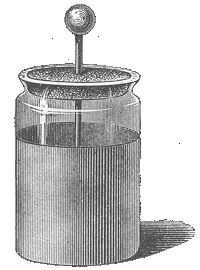
\includegraphics[width=3cm]{leidener.png}
	\caption{Leidener Flasche}
	\label{fig:leidener}
\end{wrapfigure}
In den Jahren 1745/46 versuchten zwei Forscher\footnote{1745 Ewald Georg von Kleist (Domdekan aus Cammin) und 1746 der Physiker Pieter van Musschenbroek aus Leiden} unabhängig voneinander, die beim Reiben erzeugte elektrische Ladung in Flaschen zu leiten. Man war zu dem Zeitpunkt überzeugt davon, dass es sich bei der elektrischen Ladung um irgendeine geheimnisvolle unsichtbare Flüssigkeit handeln müsse, die durch das Reiben irgendwie in Verwirbelung gebracht wurde. Anfangs klappte das nicht, die Elektrizität liess sich nicht so einfach in Flaschen abfüllen. Als man versuchte, eine Flüssigkeit in das Glas zu füllen damit die unsichtbare Ladung sich in dieser ausbreiten konnte, nahm das Experiment einen ganz anderen Verlauf: Kleist hatte bei Experimenten einen Nagel in eine alkoholgefüllte Flasche gesteckt und an eine Elektrisiermaschine angeschlossen. Beim späteren Herausziehen des Nagels erhielt er einen kräftigen elektrischen Schlag. Musschenbroek machte eine ähnliche Erfahrung.
Weitere Untersuchungen führten dann sehr schnell zur Entwicklung der ``Leidener Flasche'', dem ersten \textbf{Kondensator}. Es zeigte sich später, dass die Flüssigkeit überhaupt nicht notwendig ist und dass noch nicht einmal eine Flasche gebraucht wird. Es reicht, wenn an beiden Seiten einer flachen Scheibe aus nicht leitendem Material je eine Schicht aus leitendem Material angebracht wird (vgl. Abbildung \ref{fig:kondensator}).

\begin{center}
   \setlength{\fboxrule}{2pt}
   \fcolorbox{gray!30}{gray!10}{
\begin{minipage}{\textwidth}
\paragraph{Aufgaben}
\begin{enumerate}
\setcounter{enumi}{\value{aufgaben}}
\item Vergleichen Sie die Leidener Flasche mit dem Plattenkondensator aus dem Unterricht. Was sind die Unterschiede?
\item Was passiert auf der Aussenseite der Leidener Flasche, wenn die Innenseite positiv geladen wird?
\setcounter{aufgaben}{\value{enumi}}
\end{enumerate}
\end{minipage}
}
\end{center}


\section{Isolatoren im elektrischen Feld}
Durch ein elektrisches Feld kommt es in einem Leiter zu einer Ladungstrennung (Influenz), in einem Isolator\footnote{Nichtleiter, zum Beispiel Keramik, Glas, Kunststoff. Ein polarisierbarer Nichtleiter wird auch Dielektrikum genannt.} dagegen zu einer Polarisation. Dabei werden entweder vorhandene Dipolmoleküle\footnote{zum Beispiel Wassermoleküle} ausgerichtet, oder es finden Ladungsverschiebungen auf grösseren Molekülen statt. Während auf einer Leiteroberfläche durch ein äusseres Feld so viel Ladung verschoben wird, dass das Innere des Leiters feldfrei bleibt, schwächt die Polarisation das Feld im Innern des Nichtleiters nur etwas ab. Der Nichtleiter ist im Innern also nicht feldfrei. Bei einem Isolator in einem äusseren Feld ist also die Feldstärke im Innern des Isolators stets kleiner als die Feldstärke des äusseren Feldes. 

\begin{center}
   \setlength{\fboxrule}{2pt}
   \fcolorbox{black}{gray!10}{
\begin{minipage}{\textwidth}
\paragraph{Definition}
Die Abnahme des Felds in einem Isolator wird durch die stoffspezifische Grösse $\epsilon_{r}$ beschrieben. Diese Grösse heisst \textbf{Dielektrizitätszahl} oder auch \textbf{relative Permittivität}:
\begin{equation}
E_{in} = \frac{1}{\epsilon_{r}} \cdot E_{aeuss}
\label{defepsilonr}
\end{equation}
\end{minipage}
}
\end{center}
Die relative Permittivität $\epsilon_{r}$ eines Materials hängt davon ab, wie leicht es sich polarisieren lässt. In Tabelle \ref{tab:epsilon} sind einige Werte für $\epsilon_{r}$ aufgelistet.


\begin{figure}[h]
\begin{center}
% Sketch output, version 0.2 (build 161, Tue Sep 8 23:35:27 2009)
% Output language: PGF/TikZ,LaTeX
\begin{tikzpicture}[line join=round,scale=0.8]
\filldraw[fill=gray!30](2.449,-2.167)--(7.348,-1.167)--(4.899,.833)--(0,-.167)--cycle;
\filldraw[fill=gray!30](2.449,-2)--(7.348,-1)--(4.899,1)--(0,0)--cycle;
\filldraw[fill=blue!30](2.449,-2)--(7.348,-1)--(4.899,1)--(0,0)--cycle;
\filldraw[fill=gray!30](2.449,-.75)--(7.348,.25)--(4.899,2.25)--(0,1.25)--cycle;
\filldraw[fill=blue!30](2.449,-.75)--(7.348,.25)--(4.899,2.25)--(0,1.25)--cycle;
\filldraw[fill=gray!30](2.449,-.583)--(7.348,.417)--(4.899,2.417)--(0,1.417)--cycle;
\filldraw[fill=gray!30](0,-.167)--(2.449,-2.167)--(2.449,-2)--(0,0)--cycle;
\filldraw[fill=blue!30](0,0)--(2.449,-2)--(2.449,-.75)--(0,1.25)--cycle;
\filldraw[fill=gray!30](0,1.25)--(2.449,-.75)--(2.449,-.583)--(0,1.417)--cycle;
\filldraw[fill=gray!30](2.449,-2.167)--(7.348,-1.167)--(7.348,-1)--(2.449,-2)--cycle;
\filldraw[fill=blue!30](2.449,-2)--(7.348,-1)--(7.348,.25)--(2.449,-.75)--cycle;
\filldraw[fill=gray!30](2.449,-.75)--(7.348,.25)--(7.348,.417)--(2.449,-.583)--cycle;
\draw[<->,>=latex] (-0.2,0) -- node[left] {$d$} (-0.2,1.3);
\node [right=0.8*5cm,below=0.8*0.6cm] {$\epsilon$};
\node [right=0.8*3.5cm,above=0.8*0.6cm] {$A$};
\end{tikzpicture}% End sketch output

\caption{Kondensator mit Dielektrikum}
\label{fig:kondensator}
\end{center}
\end{figure}

Wenn nun ein Isolator zwischen den Platten eines Kondensators angebracht wird, so wird sich das elektrische Feld zwischen den Platten verkleinern. Dies führt zu einer Abnahme der Spannung zwischen den beiden Platten (vgl. Gleichung \ref{DefEplattenkondensator} auf Seite \pageref{DefEplattenkondensator}). Nach der Definition in Gleichung \ref{defkapazitaet} muss demzufolge die Kapazität des Kondensators durch den Einfluss des Isolators zunehmen. Die Gleichung \ref{Eplattenkondensator2} gilt für den Fall, dass das Feld im Kondensator nicht durch einen Isolator beeinfluss wird: $\sigma = \epsilon E_{aeuss}$. Wird nun ein Isolator in das Kondensatorfeld gebracht, bleibt die Flächenladungsdichte $\sigma$ konstant, aber die Feldstärke ändert sich: $\sigma = \epsilon \cdot \epsilon_{r} \cdot E_{in}$. Damit lässt sich die Kapazität eines Plattenkondensators für den Fall berechnen, dass der Raum zwischen seinen Platten vollständig von einem isolierenden Material ausgefüllt wird:
\begin{equation}
C = \frac{Q}{U} = \sigma \cdot \frac{A}{U}
\label{kapazitaetisolator}
\end{equation}
Mit $U = E d$ und $E = \nicefrac{\sigma}{(\epsilon \cdot \epsilon_{r}}$ ergibt sich:
\begin{equation}
C = \epsilon \cdot \epsilon_{r} \cdot \frac{A}{d}
\label{kapazitaetisolator2}
\end{equation}

\begin{figure}[h]
\begin{center}
\begin{tikzpicture}

\draw[fill=gray!30] (0,0) rectangle (1,5.1);
\draw[fill=gray!30] (9,0) rectangle (10,5.1);
\draw[fill=gray!50,draw=gray!50] (2.3,0) rectangle (7.7,5.1);
\foreach \y in {1,...,10}{
\draw[fill=white] (0.7,0.5*\y-0.2) node {$-$} circle (2mm);
\draw[fill=white] (9.3,0.5*\y-0.2) node {$+$} circle (2mm);
\draw[->,>=latex,draw=red,fill=red] (1.1,0.5*\y-0.2) -- (1.6,0.5*\y-0.2);
\draw[<-,>=latex,draw=red,fill=red] (8.4,0.5*\y-0.2) -- (8.9,0.5*\y-0.2);
\draw[<-,>=latex,draw=red,fill=red] (1.7,0.5*\y-0.2) -- (2.2,0.5*\y-0.2);
\draw[->,>=latex,draw=red,fill=red] (7.8,0.5*\y-0.2) -- (8.3,0.5*\y-0.2);
\foreach \x in {1,...,4}{
\draw[fill=gray!20] (1.9+\x*1.25,0.5*\y-0.2) node {$+ \ -$} ellipse (5mm and 2mm);
}
}
\node [right=5cm,below] {Isolator};
\end{tikzpicture}
\caption{Zwischen einem Isolator und den Kondensatorplatten kommt es zu einer Anziehung, der Isolator wird polarisiert.}
\label{Isolator}
\end{center}
\end{figure}
Dass die Kapazität $C$ eines Plattenkondensators durch den Einfluss eines polarisierbaren Isolators zunimmt, verdeutlicht auch Abbildung \ref{Isolator}. Die Ladungen auf den Kondensatorplatten werden von den polarisierten Oberflächen des Isolators angezogen. Um also eine bestimmte Ladung auf die Kondensatorplatten zu bringen, muss die anliegende Spannung nicht so gross sein wie im Falle eines Vakuums zwischen den Platten. 

\begin{center}
   \setlength{\fboxrule}{2pt}
   \fcolorbox{gray!30}{gray!10}{
\begin{minipage}{\textwidth}
\paragraph{Aufgaben}
\begin{enumerate}
\setcounter{enumi}{\value{aufgaben}}
\item Betrachten Sie Abbildung \ref{Isolator}. Weshalb kommt es zwischen dem Isolator und den Kondensatorplatten zu einer Anziehung? (Argumentieren Sie nicht mit Hilfe der Fernwirkungstheorie!)
\item Wie erklären Sie sich den grossen Unterschied zwischen den relativen Permittivitäten von Wasser und Quarzglas (vgl. Tabelle \ref{tab:epsilon})?
\setcounter{aufgaben}{\value{enumi}}
\end{enumerate}
\end{minipage}
}
\end{center}

\section{Bauformen von Kondensatoren}

Kondensatoren werden vielfältig in Stromkreisen eingesetzt, um Ladung bzw. Energie zu speichern. Aus Gleichung \ref{kapazitaetisolator2} ergibt sich, wie Kondensatoren gebaut werden müssen, damit sie eine möglichst grosse Kapazität haben, also bei einer bestimmten Spannung möglichst viel elektrische Ladung speichern können. Die Kapazität eines Kondensators ist umso grösser
\begin{itemize}
	\item je grösser die Fläche $A$ der Platten ist,
	\item je kleiner der Abstand $d$ der Platten ist,
	\item je grösser die relative Permittivität des Materials zwischen den Platten ist.
\end{itemize}

\begin{center}
   \setlength{\fboxrule}{2pt}
   \fcolorbox{gray!30}{gray!10}{
\begin{minipage}{\textwidth}
\paragraph{Aufgaben}
\begin{enumerate}
\setcounter{enumi}{\value{aufgaben}}
\item Wie ändert sich die Kapazität $C$ eines Kondensators, wenn der Abstand zwischen den Platten verdoppelt wird?
\item Zwischen zwei leitenden Metallfolien wird eine ölgetränkte Papierschicht gelegt. Das ganze wird zylinderförmig aufgewickelt. Worin bestehen die Vorteile dieses Papierkondensators?
\setcounter{aufgaben}{\value{enumi}}
\end{enumerate}
\end{minipage}
}
\end{center}

\begin{table}
\begin{center}
\begin{tabular}{|l|r|}
\hline
Stoff 				& $\epsilon_{r}$ \\
\hline
Luft  								& 1.00058 \\
Wasser 								& 80 \\
Etanol  							& 26 \\
Quarzglas 						& 3.8 \\
Porzellan  						& 6.5 \\
\hline
\end{tabular}
\caption{Relative Permittivität einiger Stoffe. Für Luft wird in der Regel der Wert $\epsilon_{r} = 1$ verwendet.}
\label{tab:epsilon}
\end{center}
\end{table}

\end{document}
